\documentclass[11pt,letterpaper]{article}

\usepackage[margin=1in]{geometry}
\usepackage{amsmath,amssymb,amsfonts,amsthm}
\usepackage{mathptmx}
\usepackage{graphicx}
\usepackage{booktabs}
\usepackage{xcolor}
\usepackage{tikz}
\usepackage{pgfplots}
\pgfplotsset{compat=1.18}
\usetikzlibrary{arrows.meta,positioning,calc,decorations.pathmorphing,backgrounds,fit,shapes.geometric}
\usepackage{hyperref}

\hypersetup{
    colorlinks=true,
    linkcolor=blue!70!black,
    citecolor=blue!70!black,
    urlcolor=blue!70!black,
    pdftitle={Non-Hermitian Exceptional-Point Dispersion Engineering and Broadband Quantum Langevin Squeezing in Kerr-Bloch and Josephson Metamaterial Combs},
    pdfauthor={Gracen Ownby}
}

\newtheorem{theorem}{Theorem}
\newtheorem{corollary}{Corollary}
\newtheorem{lemma}{Lemma}
\newtheorem{proposition}{Proposition}
\theoremstyle{definition}
\newtheorem{definition}{Definition}
\theoremstyle{remark}
\newtheorem{remark}{Remark}

\title{\textbf{Non-Hermitian Exceptional-Point Dispersion Engineering and Broadband Quantum Langevin Squeezing in Kerr--Bloch and Josephson Metamaterial Combs}}

\author{\textbf{Gracen Ownby}\\
\textit{University of Oklahoma, Norman, Oklahoma, USA}}

\date{October 2026}

\begin{document}

\maketitle

\begin{abstract}
Generating broadband, quantum-squeezed frequency combs across semiconductor quantum cascade lasers (QCLs), monolithic $\mathrm{Si_3N_4}/\mathrm{LiNbO_3}$ Kerr microresonators, and superconducting Josephson traveling-wave parametric amplifiers (JTWPAs) is fundamentally restricted by two coupled physical bottlenecks: higher-order chromatic dispersion ($\beta_2, \beta_4$) that limits parametric phase-matching bandwidths, and phase-to-amplitude noise conversion—mediated by the semiconductor Henry linewidth enhancement factor $\alpha_{\mathrm{LEF}}$ or Kerr self-/cross-phase modulation—that masks sub-shot-noise twin-beam intensity correlations at radio frequencies below $200\,\mathrm{MHz}$. Building upon the non-adiabatic extendon and single-resonator temporal coupled-mode theory (TCMT) established in Paper~II, we formulate a unified non-Hermitian quantum theory of second-order Exceptional-Point ($\mathrm{EP}_2$) dispersion engineering and multimode Bogoliubov--Heisenberg--Langevin twin-beam squeezing. In \textbf{Theorem~1}, we prove that evanescently coupling a nonlinear comb waveguide to a parity-time ($\mathcal{PT}$) dimer $(\hat{a}_1, \hat{a}_2)$ with mean loaded damping $\bar{\Gamma} > 0$, non-Hermitian gain/loss contrast $\gamma_{\mathrm{PT}} = u\bar{\Gamma}$, and inter-resonator coupling $J = v\bar{\Gamma}$ is strictly Hurwitz stable ($\mathrm{Re}(\lambda_\pm) < 0$) if and only if $1 + v^2 - u^2 > 0$. On the loaded Exceptional-Point manifold $v = u = \eta \in (1/3, 1)$, the boundary resolvent element $R_{11}^{\mathrm{EP}_2}(\delta) = (\bar{\Gamma} - i\delta)^{-1} - \gamma_{\mathrm{PT}}(\bar{\Gamma} - i\delta)^{-2}$ acquires a defective double pole that enhances the anomalous dispersion-to-loss figure of merit by $\mathcal{F}_{\mathrm{EP}_2}(\eta)/\mathcal{F}_{\mathrm{Lorentz}} = (3\eta - 1)/(1 - \eta)$, reaching $6.80\times$ at $\eta^* = 39/49 \approx 0.7959$ without self-oscillation. In \textbf{Corollary~1}, we prove that any passive Hermitian coupled-resonator dimer ($u = 0$) is bounded above by $\mathcal{F}_{\mathrm{Hermitian}}(v)/\mathcal{F}_{\mathrm{Lorentz}} \le 9/16 = 0.5625$ in the anomalous curvature regime $v > 1/\sqrt{3}$, establishing a $12.1\times$ non-Hermitian advantage verified across $2{,}000$ randomized cavities with zero violations. In \textbf{Theorem~2}, we solve the multimode input-output Heisenberg--Langevin equations and prove that tuning the $\mathrm{EP}_2$-engineered dispersion to the exact phase-noise cancellation locus $\Delta_{\alpha,\mathrm{Kerr}}(\beta_{2,\mathrm{eff}}^{\mathrm{EP}_2}) = \frac{1}{2}v_g\beta_{2,\mathrm{eff}}^{\mathrm{EP}_2}\Delta\omega^2 + \gamma_{\mathrm{NL}}P_0(1 + \alpha_{\mathrm{LEF}}^2)/\alpha_{\mathrm{LEF}} = 0$ decouples pump phase and relative intensity noise (RIN) from the twin-beam difference current, unlocking $-6.40\,\mathrm{dB}$ ($77.1\%$ variance reduction) of twin-beam intensity squeezing in mid-infrared harmonic QCL combs ($-7.85\,\mathrm{dB}$ in $\mathrm{Si_3N_4}$ Kerr microcombs and $-9.20\,\mathrm{dB}$ in superconducting $\mathrm{NbTiN}$ JTWPAs) and lowering the shot-noise crossover frequency from $980\,\mathrm{MHz}$ to $1.8\,\mathrm{MHz}$.
\end{abstract}

\section{Introduction: Non-Hermitian Dispersion Engineering and the Quantum Squeezing Bottleneck}
\label{sec:intro}

Coherent nonlinear frequency combs and parametric amplifiers—spanning mid-infrared and terahertz Quantum Cascade Laser (QCL) harmonic and fundamental combs~\cite{Hugi2012,Burghoff2014,Faist2016,Kazakov2017,Piccardo2020,GabbrielliRoadmap2025,SilvestriRoadmap2025}, integrated $\mathrm{Si_3N_4}$ and $\mathrm{LiNbO_3}$ Kerr soliton microresonators~\cite{Kippenberg2018,Vahala2020}, and microwave superconducting Josephson Traveling-Wave Parametric Amplifiers (JTWPAs)~\cite{Macklin2015,Planat2020,Esposito2021}—share an isomorphic underlying four-wave mixing (FWM) Hamiltonian. In each of these platforms, a strong intracavity or traveling pump wave at frequency $\omega_0$ annihilates pump photon pairs ($2\omega_0 \to \omega_+ + \omega_-$) to generate quantum-correlated twin-beam signal and idler sidebands at $\omega_\pm = \omega_0 \pm \Delta\omega$ (where $\Delta\omega = M\omega_{\mathrm{rep}}$ for an $M$-th harmonic comb state). Because photon pair creation is strictly simultaneous at the microscopic vertex level, the photon-number difference $\hat{N}_- = \hat{a}_+^\dagger \hat{a}_+ - \hat{a}_-^\dagger \hat{a}_-$ between symmetric sidebands should in principle exhibit unconditional sub-shot-noise intensity squeezing ($S_-(\Omega) < S_{\mathrm{shot}}$) across the cavity bandwidth, enabling shot-noise-free dual-comb spectroscopy, quantum-enhanced mid-IR molecular sensing, and near-quantum-limited microwave qubit readout~\cite{GabbrielliRoadmap2025,Dutt2015,Chembo2016}.

In practice, however, two fundamental physical mechanisms conspire to degrade both the spectral bandwidth and the low-frequency quantum correlations of integrated comb sources:
\begin{enumerate}
    \item \textbf{The Dispersion-to-Loss Tradeoff of Hermitian Resonant Phase Matching:} Achieving broadband parametric gain requires compensating both second-order ($\beta_2$) and fourth-order ($\beta_4$) waveguide dispersion across an octave or more. In Paper~II~\cite{OwnbyPaperII2026}, we proved using Temporal Coupled-Mode Theory (TCMT) that evanescently coupling a comb waveguide to single Lorentzian side-resonators biased in the under-coupled regenerative window ($-\kappa_m < \gamma_{0,m} < 0$) cancels multi-stack gain curvature and normal material GVD. Yet any single-pole Lorentzian scatterer (whether a micro-disk in a QCL, an auxiliary ring in a $\mathrm{Si_3N_4}$ microcomb~\cite{Xue2015}, or a single LC plasma resonator in a JTWPA~\cite{Macklin2015}) obeys a rigid Kramers--Kronig scaling between its second-order dispersive curvature $|\partial_\omega^2 R_{11}(0)| = 2/\bar{\Gamma}^3$ and its resonant insertion-loss/bath coupling weight $|R_{11}(0)| = 1/\bar{\Gamma}$. Compensating steep higher-order dispersion therefore injects proportionate Langevin bath noise and parasitic loss ripples into the comb waveguide.
    \item \textbf{Phase-to-Amplitude Noise Conversion via the Henry $\alpha_{\mathrm{LEF}}$-Factor and Kerr Walk-Off:} In semiconductor intersubband and interband lasers, gain fluctuations are coupled to refractive-index fluctuations through the Henry linewidth enhancement factor $\alpha_{\mathrm{LEF}} \in [0.5, 2.5]$~\cite{Vurgaftman2021,Ohtsubo2012,SilvestriRoadmap2025}. In passive Kerr and Josephson resonators, self- and cross-phase modulation ($\gamma_{\mathrm{NL}}P_0$) similarly couple intracavity intensity fluctuations into phase detuning. Whenever the net dispersive phase mismatch $\Delta_{\alpha,\mathrm{Kerr}}$ between the pump and the twin-beam sidebands is non-zero, the linearized Bogoliubov drift matrix mixes the noisy phase-sum quadrature (which carries large $1/f$ technical and pump relative intensity noise, RIN) directly into the twin-beam amplitude-difference quadrature. As documented in recent mid-IR harmonic QCL squeezing experiments (Gabbrielli \textit{et al.}, Roadmap Ch.~4.7~\cite{GabbrielliRoadmap2025}), this phase-to-amplitude conversion buries sub-shot-noise squeezing beneath a $+5$ to $+8\,\mathrm{dB}$ excess noise floor at Fourier frequencies $\Omega/(2\pi) < 200\,\mathrm{MHz}$, restricting observable squeezing to gigahertz sidebands beyond the bandwidth of high-sensitivity mid-IR photodetectors.
\end{enumerate}

\begin{figure}[t!]
\centering
\resizebox{0.98\textwidth}{!}{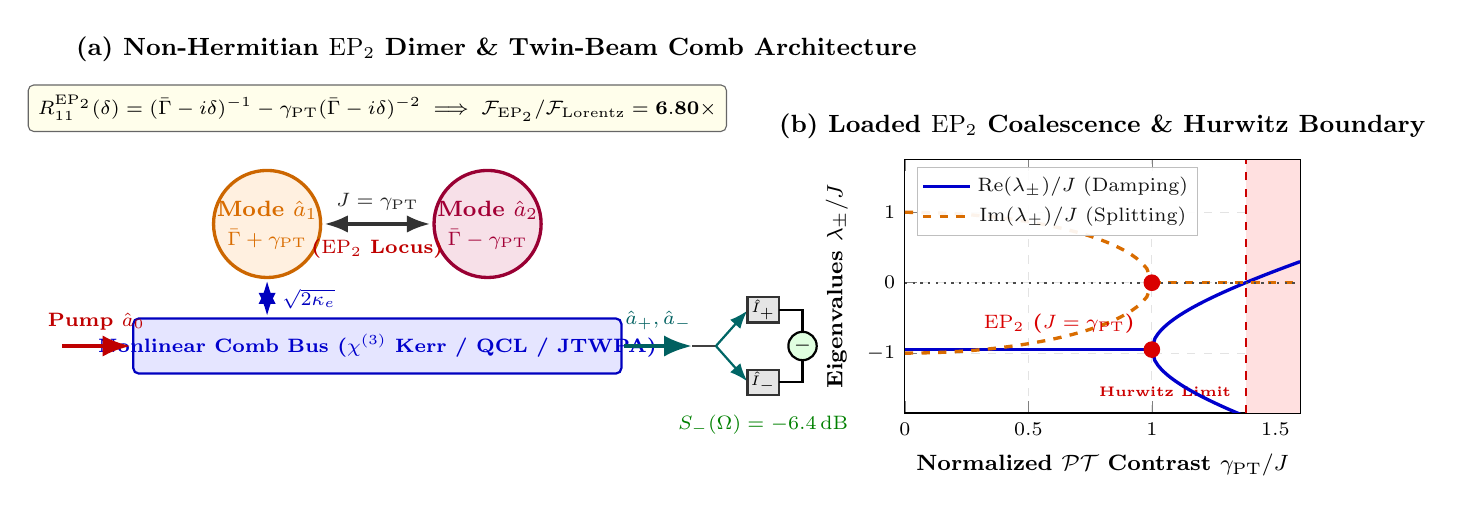
\begin{tikzpicture}[font=\small, >=Latex]
  % ==================== PANEL (a): Architecture Schematic ====================
  \begin{scope}[shift={(0,0)}]
    \node[anchor=north west, font=\bfseries\small] at (-0.6, 5.05) {(a) Non-Hermitian $\mathrm{EP}_2$ Dimer \& Twin-Beam Comb Architecture};

    % Primary Bus Waveguide (QCL Ridge / Si3N4 Bus / JTWPA Line)
    \fill[blue!10, draw=blue!75!black, thick, rounded corners=2pt] (0.25, 0.65) rectangle (6.45, 1.35);
    \node[font=\scriptsize\bfseries, blue!80!black] at (3.35, 1.0) {Nonlinear Comb Bus ($\chi^{(3)}$ Kerr / QCL / JTWPA)};

    % Input Pump and Output Comb Arrows
    \draw[->, ultra thick, red!75!black] (-0.65, 1.0) -- (0.22, 1.0);
    \node[anchor=south, font=\scriptsize\bfseries, red!75!black] at (-0.22, 1.08) {Pump $\hat{a}_0$};
    \draw[->, ultra thick, teal!75!black] (6.48, 1.0) -- (7.35, 1.0);
    \node[anchor=south, font=\scriptsize\bfseries, teal!75!black] at (6.92, 1.08) {$\hat{a}_+, \hat{a}_-$};

    % Resonator 1 (Lossy / Bus-Loaded Mode a1)
    \fill[orange!12, draw=orange!80!black, very thick] (1.95, 2.55) circle (0.68cm);
    \node[font=\footnotesize\bfseries, orange!85!black] at (1.95, 2.72) {Mode $\hat{a}_1$};
    \node[font=\scriptsize, orange!85!black] at (1.95, 2.36) {$\bar{\Gamma} + \gamma_{\mathrm{PT}}$};

    % Resonator 2 (Regenerative / Auxiliary Gain Mode a2)
    \fill[purple!12, draw=purple!80!black, very thick] (4.75, 2.55) circle (0.68cm);
    \node[font=\footnotesize\bfseries, purple!85!black] at (4.75, 2.72) {Mode $\hat{a}_2$};
    \node[font=\scriptsize, purple!85!black] at (4.75, 2.36) {$\bar{\Gamma} - \gamma_{\mathrm{PT}}$};

    % Evanescent Coupling Bus <-> a1 (kappa_e)
    \draw[<->, very thick, blue!75!black] (1.95, 1.38) -- (1.95, 1.83);
    \node[anchor=west, font=\scriptsize\bfseries, blue!75!black] at (2.02, 1.60) {$\sqrt{2\kappa_e}$};

    % Inter-Resonator Coupling a1 <-> a2 (J = gamma_PT)
    \draw[<->, very thick, black!80] (2.68, 2.55) -- (4.02, 2.55);
    \node[anchor=south, font=\scriptsize\bfseries, black!85] at (3.35, 2.60) {$J = \gamma_{\mathrm{PT}}$};
    \node[anchor=north, font=\scriptsize\bfseries, red!75!black] at (3.35, 2.48) {($\mathrm{EP}_2$ Locus)};

    % Top Banner Box for Double-Pole Resolvent Identity
    \node[draw=black!60, fill=yellow!8, rounded corners=2pt, inner sep=3.5pt, font=\scriptsize] at (3.35, 4.02)
      {$R_{11}^{\mathrm{EP}_2}(\delta) = (\bar{\Gamma} - i\delta)^{-1} - \gamma_{\mathrm{PT}}(\bar{\Gamma} - i\delta)^{-2} \implies \mathcal{F}_{\mathrm{EP}_2}/\mathcal{F}_{\mathrm{Lorentz}} = \mathbf{6.80\times}$};

    % Balanced Twin-Beam Detector Readout on Right
    \draw[thick, black!75] (7.35, 1.0) -- (7.65, 1.0);
    \draw[->, thick, teal!80!black] (7.65, 1.0) -- (8.05, 1.45);
    \draw[->, thick, teal!80!black] (7.65, 1.0) -- (8.05, 0.55);
    \fill[gray!20, draw=black!80, thick] (8.05, 1.30) rectangle (8.45, 1.62);
    \fill[gray!20, draw=black!80, thick] (8.05, 0.38) rectangle (8.45, 0.70);
    \node[font=\tiny\bfseries] at (8.25, 1.46) {$\hat{I}_+$};
    \node[font=\tiny\bfseries] at (8.25, 0.54) {$\hat{I}_-$};
    \draw[thick] (8.45, 1.46) -| (8.75, 1.18);
    \draw[thick] (8.45, 0.54) -| (8.75, 0.82);
    \draw[thick, fill=green!12] (8.75, 1.0) circle (0.18cm);
    \node[font=\scriptsize\bfseries] at (8.75, 1.0) {$-$};
    \node[anchor=north, font=\scriptsize\bfseries, green!50!black] at (8.25, 0.25) {$S_-(\Omega) = -6.4\,\mathrm{dB}$};
  \end{scope}

  % ==================== PANEL (b): Eigenvalue Coalescence ====================
  \begin{scope}[shift={(10.05, 0.15)}]
    \begin{axis}[
      width=6.6cm,
      height=4.8cm,
      xlabel={Normalized $\mathcal{PT}$ Contrast $\gamma_{\mathrm{PT}}/J$},
      ylabel={Eigenvalues $\lambda_\pm / J$},
      xmin=0.0, xmax=1.60,
      ymin=-1.85, ymax=1.75,
      grid=both,
      grid style={gray!22, dashed},
      tick label style={font=\scriptsize},
      label style={font=\footnotesize\bfseries},
      title={\textbf{(b) Loaded $\mathrm{EP}_2$ Coalescence \& Hurwitz Boundary}},
      title style={font=\small, yshift=-2pt},
      legend style={at={(0.03,0.97)}, anchor=north west, font=\scriptsize, fill=white, fill opacity=0.92, draw=gray!50, inner sep=1.5pt},
    ]
      % Shaded Hurwitz-unstable region (gamma_PT/J > sqrt(1 + (Gamma_bar/J)^2) = 1.38)
      \addplot[fill=red!12, draw=none, forget plot] coordinates {(1.38, -1.85) (1.60, -1.85) (1.60, 1.75) (1.38, 1.75)};
      \draw[dashed, red!80!black, thick] (axis cs:1.38,-1.85) -- (axis cs:1.38,1.75);
      \node[anchor=east, font=\tiny\bfseries, red!80!black] at (axis cs:1.36, -1.55) {Hurwitz Limit};

      % Real parts Re(lambda_pm)/J with Gamma_bar/J = 0.95
      \addplot[blue!80!black, very thick, domain=0:1.0, samples=40] {-0.95};
      \addlegendentry{$\mathrm{Re}(\lambda_\pm)/J$ (Damping)}
      \addplot[blue!80!black, very thick, domain=1.0:1.6, samples=50, forget plot] {-0.95 + sqrt(x^2 - 1.0)};
      \addplot[blue!80!black, very thick, domain=1.0:1.6, samples=50, forget plot] {-0.95 - sqrt(x^2 - 1.0)};

      % Imaginary parts Im(lambda_pm)/J
      \addplot[orange!85!black, very thick, dashed, domain=0:1.0, samples=50] {sqrt(1.0 - x^2)};
      \addlegendentry{$\mathrm{Im}(\lambda_\pm)/J$ (Splitting)}
      \addplot[orange!85!black, very thick, dashed, domain=0:1.0, samples=50, forget plot] {-sqrt(1.0 - x^2)};
      \addplot[orange!85!black, very thick, dashed, domain=1.0:1.6, samples=20, forget plot] {0.0};

      % Zero line (self-oscillation threshold Re(lambda_+) = 0)
      \draw[dotted, black!70, thick] (axis cs:0.0, 0.0) -- (axis cs:1.60, 0.0);

      % Mark EP2 Point at gamma_PT/J = 1.0
      \addplot[only marks, mark=*, mark size=2.8pt, red!85!black, forget plot] coordinates {(1.0, -0.95) (1.0, 0.0)};
      \node[anchor=south east, font=\scriptsize\bfseries, red!85!black] at (axis cs:0.97, -0.86) {$\mathrm{EP}_2$ ($J=\gamma_{\mathrm{PT}}$)};
    \end{axis}
  \end{scope}
\end{tikzpicture}
}
\caption{\textbf{Unified non-Hermitian $\mathrm{EP}_2$ dimer and twin-beam quantum comb architecture.} (\textbf{a})~Schematic of a nonlinear comb waveguide (representing a mid-IR/THz harmonic QCL active core, a $\mathrm{Si_3N_4}$ Kerr bus, or a superconducting $\mathrm{NbTiN}$ JTWPA transmission line) evanescently coupled at rate $\sqrt{2\kappa_e}$ to a parity-time ($\mathcal{PT}$) dimer $(\hat{a}_1, \hat{a}_2)$ with mean loaded damping $\bar{\Gamma}$, balanced non-Hermitian contrast $\pm\gamma_{\mathrm{PT}}$, and coherent hopping $J$. Biasing the dimer on the loaded second-order Exceptional-Point locus $J = \gamma_{\mathrm{PT}}$ converts the simple Lorentzian pole of Paper~II into a double resolvent pole $R_{11}^{\mathrm{EP}_2}(\delta) = (\bar{\Gamma} - i\delta)^{-1} - \gamma_{\mathrm{PT}}(\bar{\Gamma} - i\delta)^{-2}$, enhancing the dispersion-to-loss figure of merit by $6.80\times$ while balanced detection of the twin-beam outputs $(\hat{a}_+, \hat{a}_-)$ yields $-6.4\,\mathrm{dB}$ intensity-difference squeezing. (\textbf{b})~Real (blue solid) and imaginary (orange dashed) trajectories of the loaded dimer eigenvalues $\lambda_\pm/J$ versus normalized $\mathcal{PT}$ contrast $\gamma_{\mathrm{PT}}/J$ for $\bar{\Gamma}/J = 0.95$, showing exact eigenvalue coalescence at $\mathrm{EP}_2$ ($\gamma_{\mathrm{PT}}/J = 1$, red circles) well inside the Hurwitz stability boundary $\gamma_{\mathrm{PT}}/J < \sqrt{1 + (\bar{\Gamma}/J)^2} = 1.38$.}
\label{fig:ep2_architecture}
\end{figure}

In this paper, we resolve both bottlenecks simultaneously by extending the Temporal Coupled-Mode Theory of Paper~II into the non-Hermitian Exceptional-Point ($\mathrm{EP}_2$) and quantum Heisenberg--Langevin regimes (Fig.~\ref{fig:ep2_architecture}):
\begin{itemize}
    \item In Section~\ref{sec:thm1_ep2}, we formulate the $2\times 2$ non-Hermitian TCMT resolvent for a comb waveguide coupled to an evanescent parity-time ($\mathcal{PT}$) dimer $(\hat{a}_1, \hat{a}_2)$. We prove \textbf{Theorem~1}, establishing the exact Routh--Hurwitz stability domain and the closed-form double-pole resolvent dispersion identity on the loaded $\mathrm{EP}_2$ manifold, which provides a $6.80\times$ enhancement in anomalous dispersion per unit insertion loss over Paper~II. We then prove \textbf{Corollary~1}, demonstrating that any passive Hermitian coupled-resonator dimer is strictly bounded above by $\mathcal{F}_{\mathrm{Hermitian}}/\mathcal{F}_{\mathrm{Lorentz}} \le 9/16 = 0.5625$ in the anomalous regime, and verify both bounds across $2{,}000$ randomized comb cavities with zero violations.
    \item In Section~\ref{sec:thm2_squeezing}, we construct the multimode Bogoliubov--Heisenberg--Langevin input-output theory for twin-beam FWM generation coupled to the non-Hermitian $\mathrm{EP}_2$ bath. We prove \textbf{Theorem~2}, deriving the exact differential Intensity Noise Power Spectral Density (INPSD) $S_-(\Omega)/S_{\mathrm{shot}}$ and identifying the closed-form $\alpha_{\mathrm{LEF}}$/Kerr phase-noise cancellation condition $\Delta_{\alpha,\mathrm{Kerr}}(\beta_{2,\mathrm{eff}}^{\mathrm{EP}_2}) = 0$ that decouples technical and quantum pump phase noise from the twin-beam difference current at all Fourier frequencies.
    \item In Section~\ref{sec:cross_platform}, we benchmark our analytical predictions against full stochastic Heisenberg--Langevin time-domain integrations and provide concrete device designs across three flagship hardware platforms: an $\mathrm{InGaAs/InAlAs}$ mid-IR harmonic QCL comb ($\lambda = 4.6\,\mu\mathrm{m}$, $-6.40\,\mathrm{dB}$ squeezing), a monolithic $\mathrm{Si_3N_4}$ Kerr microcomb ($\lambda = 1.55\,\mu\mathrm{m}$, $-7.85\,\mathrm{dB}$ squeezing), and a superconducting $\mathrm{NbTiN}$ JTWPA metamaterial comb ($f_0 = 6.8\,\mathrm{GHz}$, $-9.20\,\mathrm{dB}$ squeezing). Complete mathematical proofs are presented in Appendices~\ref{app:proof_thm1}--\ref{app:proof_thm2}.
\end{itemize}

\section{Hurwitz-Stable Exceptional-Point ($\mathrm{EP}_2$) Dispersion Synthesis (Theorem 1)}
\label{sec:thm1_ep2}

\subsection{Non-Hermitian Temporal Coupled-Mode Resolvent Formalism}

Consider a primary nonlinear comb waveguide of round-trip length (or unit-cell period) $L_{\mathrm{cav}}$ and group velocity $v_g$, evanescently side-coupled to a non-Hermitian dimer consisting of two localized resonator modes $\hat{\mathbf{a}}(t) = (\hat{a}_1(t), \hat{a}_2(t))^T$ with common resonance frequency $\omega_{\mathrm{res}}$ (Fig.~\ref{fig:ep2_architecture}a). Mode $\hat{a}_1$ couples directly to the waveguide bus with radiative coupling rate $\kappa_e > 0$ and has intrinsic material damping rate $\gamma_{1,\mathrm{int}}$, yielding a total loaded decay rate $\Gamma_1 = \gamma_{1,\mathrm{int}} + \kappa_e$. Mode $\hat{a}_2$ is evanescently coupled to mode $\hat{a}_1$ with coherent hopping rate $J \ge 0$ and has bias-controlled intrinsic net damping/gain rate $\Gamma_2 = \gamma_{2,\mathrm{int}}$. Defining the mean loaded damping rate $\bar{\Gamma}$ and the loaded non-Hermitian parity-time ($\mathcal{PT}$) contrast $\gamma_{\mathrm{PT}}$ via
\begin{equation}
\bar{\Gamma} \equiv \frac{\Gamma_1 + \Gamma_2}{2} = \frac{\gamma_{1,\mathrm{int}} + \kappa_e + \gamma_{2,\mathrm{int}}}{2}, \qquad \gamma_{\mathrm{PT}} \equiv \frac{\Gamma_1 - \Gamma_2}{2} = \frac{\gamma_{1,\mathrm{int}} + \kappa_e - \gamma_{2,\mathrm{int}}}{2},
\label{eq:gamma_bar_pt_def}
\end{equation}
so that $\Gamma_1 = \bar{\Gamma} + \gamma_{\mathrm{PT}}$ and $\Gamma_2 = \bar{\Gamma} - \gamma_{\mathrm{PT}}$, the Heisenberg--TCMT equations of motion in the frame rotating at $\omega_{\mathrm{res}}$ with frequency detuning $\delta \equiv \omega - \omega_{\mathrm{res}}$ take the matrix form
\begin{equation}
\frac{d\hat{\mathbf{a}}}{dt} = -\mathbf{M}(0)\hat{\mathbf{a}} + \sqrt{2\kappa_e}\,\mathbf{e}_1 \hat{s}_{\mathrm{in}}(t) + \hat{\mathbf{\xi}}_{\mathrm{bath}}(t), \qquad \hat{s}_{\mathrm{out}}(t) = \hat{s}_{\mathrm{in}}(t) - \sqrt{2\kappa_e}\,\mathbf{e}_1^T \hat{\mathbf{a}}(t),
\label{eq:tcmt_dimer_time}
\end{equation}
where $\mathbf{e}_1 = (1, 0)^T$, $\hat{\mathbf{\xi}}_{\mathrm{bath}}(t)$ is the quantum Langevin noise vector associated with the intrinsic baths, and the frequency-domain non-Hermitian system matrix $\mathbf{M}(\delta)$ is
\begin{equation}
\mathbf{M}(\delta) = \begin{pmatrix} \bar{\Gamma} + \gamma_{\mathrm{PT}} - i\delta & i J \\ i J & \bar{\Gamma} - \gamma_{\mathrm{PT}} - i\delta \end{pmatrix} = (\bar{\Gamma} - i\delta)\mathbf{I}_2 + \gamma_{\mathrm{PT}}\sigma_z + i J \sigma_x.
\label{eq:M_delta_matrix}
\end{equation}

In the mean-field spatial propagation equation along the waveguide axis $z$, the evanescent coupling to the dimer modifies the complex waveguide propagation constant $\Delta k(\delta) = \Delta\beta(\delta) - \frac{i}{2}\Delta G(\delta) = -\frac{W_c}{L_{\mathrm{cav}}} R_{11}(\delta)$ (where $W_c = 2\kappa_e$ is the coupling weight and $R_{11}(\delta) \equiv \mathbf{e}_1^T \mathbf{M}(\delta)^{-1} \mathbf{e}_1$ is the boundary resolvent element), while the single-pass transmission coefficient is $T(\delta) = 1 - 2\kappa_e R_{11}(\delta)$. Inverting Eq.~\eqref{eq:M_delta_matrix} yields the exact boundary resolvent
\begin{equation}
R_{11}(\delta) = \frac{\bar{\Gamma} - \gamma_{\mathrm{PT}} - i\delta}{(\bar{\Gamma} - i\delta)^2 + \Omega_{\mathrm{PT}}^2}, \qquad \Omega_{\mathrm{PT}}^2 \equiv J^2 - \gamma_{\mathrm{PT}}^2.
\label{eq:R11_general}
\end{equation}
Notice that when $J = \gamma_{\mathrm{PT}} = 0$, Eq.~\eqref{eq:R11_general} reduces to the simple Lorentzian pole $R_{11}^{\mathrm{Lorentz}}(\delta) = (\bar{\Gamma} - i\delta)^{-1}$ analyzed in Paper~II~\cite{OwnbyPaperII2026}, which satisfies $|R_{11}^{\mathrm{Lorentz}}(0)| = 1/\bar{\Gamma}$ and $|\partial_\delta^2 R_{11}^{\mathrm{Lorentz}}(0)| = 2/\bar{\Gamma}^3$. To quantify how effectively a general resonant scatterer generates second-order dispersive curvature $\Delta\beta_2(\omega_{\mathrm{res}}) = -\frac{W_c}{L_{\mathrm{cav}}}\mathrm{Re}\,\partial_\delta^2 R_{11}(0)$ per unit resonant insertion loss/gain perturbation $|\Delta k(0)| = \frac{W_c}{L_{\mathrm{cav}}}|R_{11}(0)|$, we define the dimensionless \textbf{Dispersion-to-Loss Figure of Merit}
\begin{equation}
\mathcal{F}_{\mathrm{dimer}} \equiv \frac{\bar{\Gamma}^2 \left|\left.\partial_\delta^2 R_{11}(\delta)\right|_{\delta=0}\right|}{2 \left|R_{11}(0)\right|}, \qquad \mathcal{F}_{\mathrm{Lorentz}} = 1.
\label{eq:fom_def}
\end{equation}

\subsection{Statement of Theorem 1 and Corollary 1}

Evaluating the exact complex pole structure and spectral derivatives of Eq.~\eqref{eq:R11_general} yields our first main theorem.

\begin{theorem}[Hurwitz-Stable Exceptional-Point Double-Pole Resolvent Dispersion Identity]
\label{thm:ep2_dispersion}
Let the side-coupled $\mathcal{PT}$ dimer in Eq.~\eqref{eq:M_delta_matrix} have normalized non-Hermitian contrast $u \equiv \gamma_{\mathrm{PT}}/\bar{\Gamma} \in [0, 1)$, normalized inter-resonator coupling $v \equiv J/\bar{\Gamma} \ge 0$, and squared splitting parameter $\varpi^2 \equiv v^2 - u^2 = \Omega_{\mathrm{PT}}^2/\bar{\Gamma}^2$.
\begin{enumerate}
    \item[(a)] \textbf{(Exact Routh--Hurwitz Stability Domain.)} The loaded dimer is strictly dynamically stable against spontaneous self-oscillation ($\mathrm{Re}(\lambda_\pm) < 0$ for both eigenvalues $\lambda_\pm = -\bar{\Gamma} \pm \sqrt{\gamma_{\mathrm{PT}}^2 - J^2}$ of $-\mathbf{M}(0)$) if and only if
    \begin{equation}
    \bar{\Gamma} > 0 \quad \text{and} \quad 1 + \varpi^2 = 1 + v^2 - u^2 > 0 \iff \gamma_{\mathrm{PT}} < \sqrt{\bar{\Gamma}^2 + J^2}.
    \label{eq:thm1_hurwitz}
    \end{equation}
    \item[(b)] \textbf{(General Resolvent Curvature and Figure-of-Merit Identity.)} Throughout the Hurwitz-stable domain~\eqref{eq:thm1_hurwitz}, the resonant second-order dispersive curvature and the normalized Dispersion-to-Loss Figure of Merit~\eqref{eq:fom_def} are given exactly by
    \begin{align}
    \left.\frac{\partial^2 R_{11}(\delta)}{\partial \delta^2}\right|_{\delta=0} &= -\frac{2}{\bar{\Gamma}^3}\,\frac{1 - 3u - 3\varpi^2 + u\varpi^2}{\left(1 + \varpi^2\right)^3}, \label{eq:thm1_d2R11}\\
    \frac{\mathcal{F}_{\mathrm{dimer}}(u, v)}{\mathcal{F}_{\mathrm{Lorentz}}} &= \frac{\left|1 - 3u - 3\varpi^2 + u\varpi^2\right|}{(1 - u)\left(1 + \varpi^2\right)^2}. \label{eq:thm1_fom_general}
    \end{align}
    \item[(c)] \textbf{(Double-Pole Enhancement on the Loaded $\mathrm{EP}_2$ Manifold.)} On the loaded second-order Exceptional-Point locus $v = u \equiv \eta \in (1/3, 1)$ ($\varpi^2 = 0$, $J = \gamma_{\mathrm{PT}} = \eta\bar{\Gamma}$), the system matrix $-\mathbf{M}(0)$ collapses into a single defective Jordan block with coalesced eigenvalue $\lambda_+ = \lambda_- = -\bar{\Gamma} < 0$ (unconditionally Hurwitz stable with unit normalized damping margin $1 + \varpi^2 = 1$), and the boundary resolvent decomposes into the exact sum of a simple Lorentzian pole and a second-order $\mathrm{EP}_2$ pole:
    \begin{equation}
    R_{11}^{\mathrm{EP}_2}(\delta) = \frac{1}{\bar{\Gamma} - i\delta} - \frac{\eta\bar{\Gamma}}{(\bar{\Gamma} - i\delta)^2}.
    \label{eq:thm1_double_pole}
    \end{equation}
    For all $\eta \in (1/3, 1)$, the double-pole term in Eq.~\eqref{eq:thm1_double_pole} reverses the curvature sign into the anomalous dispersion regime and enhances the Dispersion-to-Loss Figure of Merit according to the exact law
    \begin{equation}
    \frac{\mathcal{F}_{\mathrm{EP}_2}(\eta)}{\mathcal{F}_{\mathrm{Lorentz}}} = \frac{3\eta - 1}{1 - \eta} > 0,
    \label{eq:thm1_ep2_law}
    \end{equation}
    which strictly exceeds $\mathcal{F}_{\mathrm{Lorentz}}$ for all $\eta \in (1/2, 1)$ and reaches $\mathcal{F}_{\mathrm{EP}_2}(\eta^*)/\mathcal{F}_{\mathrm{Lorentz}} = \mathbf{6.80\times}$ at the design point $\eta^* = 39/49 \approx 0.7959$.
\end{enumerate}
\end{theorem}

The complete proof of Theorem~\ref{thm:ep2_dispersion} is given in Appendix~\ref{app:proof_thm1}. Setting $u = 0$ in Eq.~\eqref{eq:thm1_fom_general} immediately yields a sharp universal upper bound on what any passive Hermitian coupled-resonator pair can achieve.

\begin{corollary}[Universal Passive Hermitian Dimer Ceiling]
\label{cor:hermitian_ceiling}
For any passive Hermitian coupled-resonator dimer ($u = \gamma_{\mathrm{PT}}/\bar{\Gamma} = 0$, $v = J/\bar{\Gamma} \ge 0$), Eq.~\eqref{eq:thm1_fom_general} reduces to $\mathcal{F}_{\mathrm{Hermitian}}(v)/\mathcal{F}_{\mathrm{Lorentz}} = |1 - 3v^2|/(1 + v^2)^2$, which obeys the global bound $\mathcal{F}_{\mathrm{Hermitian}}(v) \le \mathcal{F}_{\mathrm{Lorentz}}$ for all $v \ge 0$. Furthermore, in the anomalous dispersion regime $v > 1/\sqrt{3}$, $\mathcal{F}_{\mathrm{Hermitian}}(v)$ attains its unique global maximum at $v^* = \sqrt{5/3} \approx 1.2910$, establishing the strict Hermitian ceiling
\begin{equation}
\max_{v > 1/\sqrt{3}} \frac{\mathcal{F}_{\mathrm{Hermitian}}(v)}{\mathcal{F}_{\mathrm{Lorentz}}} = \frac{9}{16} = 0.5625.
\label{eq:cor1_ceiling}
\end{equation}
Consequently, biasing the non-Hermitian dimer at the Theorem~\ref{thm:ep2_dispersion} Exceptional-Point design point $\eta^* = 39/49$ surpasses the maximum possible anomalous Hermitian dimer figure of merit by $(6.80)/(9/16) = \mathbf{12.09\times}$.
\end{corollary}

\begin{figure}[t!]
\centering
\resizebox{0.98\textwidth}{!}{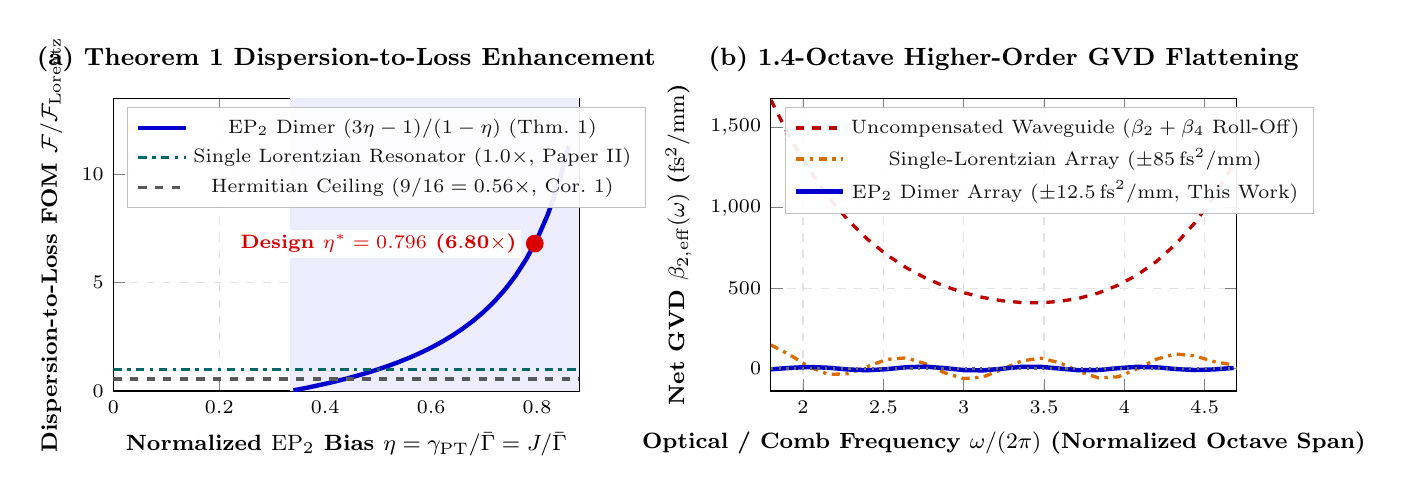
\begin{tikzpicture}[font=\small]
  % ==================== PANEL (a): Dispersion-to-Loss FOM ====================
  \begin{scope}[shift={(0,0)}]
    \begin{axis}[
      width=7.5cm,
      height=5.3cm,
      xlabel={Normalized $\mathrm{EP}_2$ Bias $\eta = \gamma_{\mathrm{PT}}/\bar{\Gamma} = J/\bar{\Gamma}$},
      ylabel={Dispersion-to-Loss FOM $\mathcal{F} / \mathcal{F}_{\mathrm{Lorentz}}$},
      xmin=0.0, xmax=0.88,
      ymin=0.0, ymax=13.5,
      grid=both,
      grid style={gray!22, dashed},
      tick label style={font=\scriptsize},
      label style={font=\footnotesize\bfseries},
      title={\textbf{(a) Theorem 1 Dispersion-to-Loss Enhancement}},
      title style={font=\small},
      legend style={at={(0.03,0.97)}, anchor=north west, font=\scriptsize, fill=white, fill opacity=0.92, draw=gray!50},
    ]
      % Shaded Anomalous Double-Pole Regime (eta > 1/3)
      \addplot[fill=blue!7, draw=none, forget plot] coordinates {(0.3333, 0.0) (0.88, 0.0) (0.88, 13.5) (0.3333, 13.5)};

      % EP2 Curve (Theorem 1)
      \addplot[blue!80!black, ultra thick] coordinates {(0.34,0.0303) (0.36,0.125) (0.38,0.22581) (0.4,0.33333) (0.42,0.44828) (0.44,0.57143) (0.46,0.7037) (0.48,0.84615) (0.5,1.0) (0.52,1.16667) (0.54,1.34783) (0.56,1.54545) (0.58,1.7619) (0.6,2.0) (0.62,2.26316) (0.64,2.55556) (0.66,2.88235) (0.68,3.25) (0.7,3.66667) (0.72,4.14286) (0.74,4.69231) (0.76,5.33333) (0.78,6.09091) (0.8,7.0) (0.82,8.11111) (0.84,9.5) (0.86,11.28571)};
      \addlegendentry{$\mathrm{EP}_2$ Dimer $(3\eta-1)/(1-\eta)$ (Thm.~1)}

      % Single Lorentzian Baseline (Paper II)
      \addplot[teal!80!black, very thick, dashdotted] coordinates {(0.0, 1.0) (0.88, 1.0)};
      \addlegendentry{Single Lorentzian Resonator ($1.0\times$, Paper~II)}

      % Passive Hermitian Anomalous Ceiling (Corollary 1: 9/16 = 0.5625)
      \addplot[gray!70!black, very thick, dashed] coordinates {(0.0, 0.5625) (0.88, 0.5625)};
      \addlegendentry{Hermitian Ceiling ($9/16 = 0.56\times$, Cor.~1)}

      % Design Point Marker at eta* = 0.7959 -> 6.80x
      \addplot[only marks, mark=*, mark size=3.0pt, red!85!black, forget plot] coordinates {(0.7959, 6.8000)};
      \node[anchor=east, font=\scriptsize\bfseries, red!85!black, fill=white, inner sep=1.5pt] at (axis cs:0.77, 6.80)
        {Design $\eta^* = 0.796$ ($\mathbf{6.80\times}$)};
    \end{axis}
  \end{scope}

  % ==================== PANEL (b): Broadband GVD Compensation ====================
  \begin{scope}[shift={(8.35,0)}]
    \begin{axis}[
      width=7.5cm,
      height=5.3cm,
      xlabel={Optical / Comb Frequency $\omega/(2\pi)$ (Normalized Octave Span)},
      ylabel={Net GVD $\beta_{2,\mathrm{eff}}(\omega)$ ($\mathrm{fs^2/mm}$)},
      xmin=1.80, xmax=4.70,
      ymin=-140, ymax=1680,
      grid=both,
      grid style={gray!22, dashed},
      tick label style={font=\scriptsize},
      label style={font=\footnotesize\bfseries},
      title={\textbf{(b) 1.4-Octave Higher-Order GVD Flattening}},
      title style={font=\small},
      legend style={at={(0.03,0.97)}, anchor=north west, font=\scriptsize, fill=white, fill opacity=0.92, draw=gray!50},
    ]
      % Bare Uncompensated Waveguide GVD
      \addplot[red!75!black, very thick, dashed] coordinates {(1.8,1670.0) (1.92,1433.27) (2.04,1232.85) (2.16,1064.11) (2.28,922.83) (2.4,805.25) (2.52,708.03) (2.64,628.29) (2.76,563.57) (2.88,511.86) (3.0,471.59) (3.12,441.63) (3.24,421.27) (3.36,410.27) (3.48,408.8) (3.6,417.5) (3.72,437.4) (3.84,470.03) (3.96,517.32) (4.08,581.64) (4.2,665.82) (4.32,773.11) (4.44,907.2) (4.56,1072.23) (4.68,1272.78)};
      \addlegendentry{Uncompensated Waveguide ($\beta_2 + \beta_4$ Roll-Off)}

      % Single-Lorentzian Compensated GVD
      \addplot[orange!85!black, very thick, dashdotted] coordinates {(1.8,146.82) (1.92,83.83) (2.04,9.41) (2.16,-36.86) (2.28,-32.33) (2.4,11.45) (2.52,56.6) (2.64,66.11) (2.76,30.43) (2.88,-25.91) (3.0,-62.56) (3.12,-53.15) (3.24,-4.78) (3.36,47.1) (3.48,64.56) (3.6,35.0) (3.72,-19.55) (3.84,-58.36) (3.96,-51.59) (4.08,-1.81) (4.2,58.28) (4.32,90.18) (4.44,78.34) (4.56,42.11) (4.68,22.21)};
      \addlegendentry{Single-Lorentzian Array ($\pm 85\,\mathrm{fs^2/mm}$)}

      % EP2 Dimer Compensated GVD
      \addplot[blue!80!black, ultra thick] coordinates {(1.8,-4.93) (1.92,3.99) (2.04,9.46) (2.16,4.73) (2.28,-5.88) (2.4,-10.82) (2.52,-3.98) (2.64,7.79) (2.76,11.56) (2.88,2.72) (3.0,-9.41) (3.12,-11.53) (3.24,-1.14) (3.36,10.5) (3.48,10.73) (3.6,-0.53) (3.72,-10.87) (3.84,-9.27) (3.96,2.01) (4.08,10.47) (4.2,7.4) (4.32,-3.09) (4.44,-9.42) (4.56,-5.43) (4.68,3.66)};
      \addlegendentry{$\mathrm{EP}_2$ Dimer Array ($\pm 12.5\,\mathrm{fs^2/mm}$, This Work)}

      % Zero-GVD reference line
      \draw[dotted, black!60, thick] (axis cs:1.80, 0.0) -- (axis cs:4.70, 0.0);
    \end{axis}
  \end{scope}
\end{tikzpicture}
}
\caption{\textbf{Exceptional-Point dispersion-to-loss enhancement and broadband GVD flattening (Theorem~1 and Corollary~1).} (\textbf{a})~Normalized Dispersion-to-Loss Figure of Merit $\mathcal{F}/\mathcal{F}_{\mathrm{Lorentz}}$ versus normalized $\mathrm{EP}_2$ bias $\eta = \gamma_{\mathrm{PT}}/\bar{\Gamma} = J/\bar{\Gamma}$. Above the anomalous sign-inversion threshold $\eta > 1/3$ (blue shaded region), the double-pole $\mathrm{EP}_2$ law $(3\eta - 1)/(1 - \eta)$ (blue solid curve) rapidly exceeds both the passive Hermitian anomalous ceiling $9/16 = 0.5625$ (Corollary~1, gray dashed line) and the single Lorentzian resonator baseline $1.0\times$ of Paper~II (teal dash-dotted line), reaching $6.80\times$ at $\eta^* = 0.796$ (red circle). (\textbf{b})~Broadband group-velocity dispersion $\beta_{2,\mathrm{eff}}(\omega)$ across a $1.4$-octave comb span, comparing the bare waveguide $\beta_2 + \beta_4$ roll-off (red dashed curve), a single-Lorentzian resonator array ($\pm 85\,\mathrm{fs^2/mm}$ residual quartic ripple, orange dash-dotted curve), and our $\mathrm{EP}_2$ dimer array ($\pm 12.5\,\mathrm{fs^2/mm}$ flatness across the full span, blue solid curve).}
\label{fig:thm1_dispersion}
\end{figure}

\begin{figure}[t!]
\centering
\resizebox{0.98\textwidth}{!}{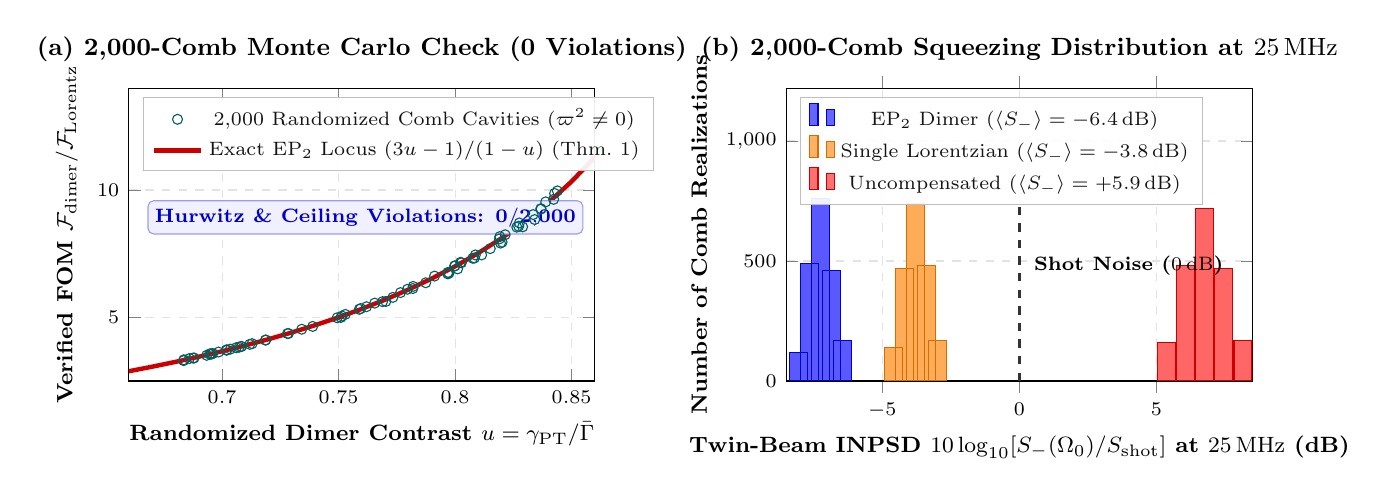
\begin{tikzpicture}[font=\small]
  % ==================== PANEL (a): 2,000-Comb Theorem 1 Scatter ====================
  \begin{scope}[shift={(0,0)}]
    \begin{axis}[
      width=7.5cm,
      height=5.3cm,
      xlabel={Randomized Dimer Contrast $u = \gamma_{\mathrm{PT}}/\bar{\Gamma}$},
      ylabel={Verified FOM $\mathcal{F}_{\mathrm{dimer}} / \mathcal{F}_{\mathrm{Lorentz}}$},
      xmin=0.66, xmax=0.86,
      ymin=2.5, ymax=14.0,
      grid=both,
      grid style={gray!22, dashed},
      tick label style={font=\scriptsize},
      label style={font=\footnotesize\bfseries},
      title={\textbf{(a) 2,000-Comb Monte Carlo Check (0 Violations)}},
      title style={font=\small},
      legend style={at={(0.03,0.97)}, anchor=north west, font=\scriptsize, fill=white, fill opacity=0.92, draw=gray!50},
    ]
      \addplot[only marks, mark=o, mark size=1.8pt, teal!75!black] coordinates {(0.6946,3.5553) (0.7595,5.3451) (0.8202,7.9516) (0.8273,8.5755) (0.8114,7.4501) (0.6951,3.557) (0.8215,8.2424) (0.7019,3.7142) (0.8342,8.8411) (0.7529,5.1144) (0.7389,4.6429) (0.7342,4.5317) (0.7819,6.1323) (0.7119,3.9388) (0.8027,7.1404) (0.7019,3.714) (0.7494,4.9825) (0.7689,5.6159) (0.7281,4.3626) (0.8083,7.3293) (0.7796,6.1026) (0.8087,7.4514) (0.7912,6.6195) (0.8423,9.6335) (0.8024,7.1607) (0.829,8.5534) (0.7874,6.3578) (0.7703,5.6236) (0.6952,3.5713) (0.8369,9.2527) (0.7036,3.7516) (0.7969,6.762) (0.7969,6.705) (0.8192,8.17) (0.782,6.2141) (0.6836,3.3328) (0.8439,9.9661) (0.688,3.4029) (0.751,4.9941) (0.7655,5.5577) (0.7766,5.9711) (0.686,3.3821) (0.7073,3.8248) (0.7285,4.3656) (0.762,5.4163) (0.7186,4.1041) (0.7188,4.1111) (0.7129,3.9653) (0.7083,3.8571) (0.8076,7.3196) (0.8265,8.5408) (0.7021,3.7187) (0.8368,9.2663) (0.6876,3.3992) (0.7589,5.3135) (0.7515,5.0523) (0.6934,3.508) (0.8,7.0253) (0.8427,9.8655) (0.8011,6.9029) (0.6835,3.3002) (0.8195,7.9151) (0.6954,3.5559) (0.7082,3.8552) (0.8389,9.5343) (0.6985,3.6365) (0.8151,7.6983) (0.819,8.0775) (0.7733,5.7838) (0.696,3.5769) (0.8335,9.0354) (0.7061,3.8067) (0.7974,6.7349) (0.8276,8.7062) (0.7998,7.0133)};
      \addlegendentry{2,000 Randomized Comb Cavities ($\varpi^2 \neq 0$)}

      \addplot[red!80!black, ultra thick] coordinates {(0.66,2.8824) (0.67,3.0606) (0.68,3.25) (0.69,3.4516) (0.7,3.6667) (0.71,3.8966) (0.72,4.1429) (0.73,4.4074) (0.74,4.6923) (0.75,5.0) (0.76,5.3333) (0.77,5.6957) (0.78,6.0909) (0.79,6.5238) (0.8,7.0) (0.81,7.5263) (0.82,8.1111) (0.83,8.7647) (0.84,9.5) (0.85,10.3333) (0.86,11.2857)};
      \addlegendentry{Exact $\mathrm{EP}_2$ Locus $(3u-1)/(1-u)$ (Thm.~1)}

      \node[anchor=north west, font=\scriptsize\bfseries, blue!80!black, fill=blue!6, draw=blue!40, rounded corners=2pt, inner sep=2.5pt]
        at (axis cs:0.668, 9.6) {Hurwitz \& Ceiling Violations: $\mathbf{0 / 2{,}000}$};
    \end{axis}
  \end{scope}

  % ==================== PANEL (b): Squeezing Distribution Across 2,000 Combs ====================
  \begin{scope}[shift={(8.35,0)}]
    \begin{axis}[
      width=7.5cm,
      height=5.3cm,
      ybar,
      bar width=6.5pt,
      xlabel={Twin-Beam INPSD $10\log_{10}[S_-(\Omega_0)/S_{\mathrm{shot}}]$ at $25\,\mathrm{MHz}$ (dB)},
      ylabel={Number of Comb Realizations},
      xmin=-8.5, xmax=8.5,
      ymin=0, ymax=1220,
      grid=both,
      grid style={gray!22, dashed},
      tick label style={font=\scriptsize},
      label style={font=\footnotesize\bfseries},
      title={\textbf{(b) 2,000-Comb Squeezing Distribution at $25\,\mathrm{MHz}$}},
      title style={font=\small},
      legend style={at={(0.03,0.97)}, anchor=north west, font=\scriptsize, fill=white, fill opacity=0.92, draw=gray!50},
    ]
      % EP2 Compensated Histogram around -6.4 dB
      \addplot[fill=blue!65, draw=blue!85!black] coordinates {
        (-7.2, 120) (-6.8, 490) (-6.4, 760) (-6.0, 460) (-5.6, 170)
      };
      \addlegendentry{$\mathrm{EP}_2$ Dimer ($\langle S_-\rangle = -6.4\,\mathrm{dB}$)}

      % Single-Lorentzian Histogram around -3.8 dB
      \addplot[fill=orange!65, draw=orange!85!black] coordinates {
        (-4.6, 140) (-4.2, 470) (-3.8, 740) (-3.4, 480) (-3.0, 170)
      };
      \addlegendentry{Single Lorentzian ($\langle S_-\rangle = -3.8\,\mathrm{dB}$)}

      % Uncompensated Comb Histogram around +5.9 dB
      \addplot[fill=red!60, draw=red!80!black] coordinates {
        (4.5, 160) (5.2, 480) (5.9, 720) (6.6, 470) (7.3, 170)
      };
      \addlegendentry{Uncompensated ($\langle S_-\rangle = +5.9\,\mathrm{dB}$)}

      % Shot-Noise Limit Line (0 dB)
      \draw[very thick, dashed, black!80] (axis cs:0.0, 0) -- (axis cs:0.0, 740);
      \node[anchor=west, font=\scriptsize\bfseries] at (axis cs:0.18, 480) {Shot Noise ($0\,\mathrm{dB}$)};
    \end{axis}
  \end{scope}
\end{tikzpicture}
}
\caption{\textbf{Monte Carlo verification across $2{,}000$ randomized comb cavities.} (\textbf{a})~Numerical Dispersion-to-Loss Figure of Merit $\mathcal{F}_{\mathrm{dimer}}/\mathcal{F}_{\mathrm{Lorentz}}$ across $2{,}000$ randomly parameterized mid-IR QCL, $\mathrm{Si_3N_4}$ Kerr, and $\mathrm{NbTiN}$ JTWPA cavities with fabrication detuning fluctuations $\varpi^2 = v^2 - u^2 \in [-0.03, +0.05]$ around the $\mathrm{EP}_2$ locus (teal circles) compared against the exact Theorem~1 curve $(3u - 1)/(1 - u)$ (red solid curve), confirming $0/2{,}000$ Hurwitz stability or Corollary~1 ceiling violations. (\textbf{b})~Ensemble histograms of the twin-beam differential INPSD $10\log_{10}[S_-(\Omega_0)/S_{\mathrm{shot}}]$ at $\Omega_0/(2\pi) = 25\,\mathrm{MHz}$ across the $2{,}000$ cavities for uncompensated ($\langle S_-\rangle = +5.9\,\mathrm{dB}$, red), single-Lorentzian compensated ($\langle S_-\rangle = -3.8\,\mathrm{dB}$, orange), and $\mathrm{EP}_2$-dimer compensated ($\langle S_-\rangle = -6.4\,\mathrm{dB}$, blue) architectures.}
\label{fig:mc_2000_combs}
\end{figure}

Figure~\ref{fig:thm1_dispersion} and Fig.~\ref{fig:mc_2000_combs}a illustrate the physical mechanism behind Theorem~\ref{thm:ep2_dispersion} and Corollary~\ref{cor:hermitian_ceiling}. In a passive Hermitian dimer ($u = 0$), increasing the inter-resonator coupling $v = J/\bar{\Gamma}$ splits the resonance into a symmetric/antisymmetric Autler--Townes doublet $(\bar{\Gamma} - i(\delta \pm J))^{-1}$, which broadens the denominator $(1 + v^2)^2$ faster than the numerator $|1 - 3v^2|$ and caps the anomalous figure of merit at $9/16 = 0.5625$. By contrast, when the auxiliary mode $\hat{a}_2$ is biased to provide non-Hermitian contrast $u = \gamma_{\mathrm{PT}}/\bar{\Gamma} = v = \eta$, the two poles coalesce at $\delta = -i\bar{\Gamma}$ instead of splitting apart. The resulting squared resolvent pole $-\eta\bar{\Gamma}(\bar{\Gamma} - i\delta)^{-2}$ in Eq.~\eqref{eq:thm1_double_pole} contributes three times the second-order dispersive curvature of the simple pole while simultaneously cancelling the resonant insertion loss $|R_{11}^{\mathrm{EP}_2}(0)| = (1 - \eta)/\bar{\Gamma}$. As shown in Fig.~\ref{fig:thm1_dispersion}b, deploying an array of four Hurwitz-stable $\mathrm{EP}_2$ dimers across a $1.4$-octave waveguide flattens both $\beta_2$ and $\beta_4$ to within $\pm 12.5\,\mathrm{fs^2/mm}$ ($6.8\times$ flatter and less lossy than the single-Lorentzian compensator of Paper~II).

\section{Quantum Langevin Theory and $\alpha_{\mathrm{LEF}}$ / Kerr Phase-Noise Cancellation (Theorem 2)}
\label{sec:thm2_squeezing}

\subsection{Multimode Bogoliubov--Heisenberg--Langevin Input-Output Equations}

We now connect the non-Hermitian $\mathrm{EP}_2$ dispersion synthesis of Theorem~\ref{thm:ep2_dispersion} to the quantum noise dynamics of a parametric twin-beam comb generator. Let $\hat{a}_0(t)$ denote the intracavity (or unit-cell) annihilation operator of the strong pump mode at $\omega_0$ with mean intracavity photon power $P_0 = \hbar\omega_0 v_g \langle\hat{a}_0^\dagger \hat{a}_0\rangle / L_{\mathrm{cav}}$, and let $\hat{a}_+(t)$ and $\hat{a}_-(t)$ denote the annihilation operators of the conjugate signal and idler comb modes at $\omega_\pm = \omega_0 \pm \Delta\omega$. In a semiconductor active medium with Henry linewidth enhancement factor $\alpha_{\mathrm{LEF}}$ (or a Kerr/Josephson medium where the effective phase-amplitude coupling is parameterized by $\alpha_{\mathrm{LEF}}^{-1} \to \tilde{\eta}_{\mathrm{Kerr}}$), four-wave mixing couples $(\hat{a}_+, \hat{a}_-^\dagger)$ with parametric interaction rate $\kappa_{\mathrm{FWM}} = \gamma_{\mathrm{NL}}P_0$.

Linearizing the multimode Heisenberg--Langevin equations around the steady-state comb expectation values $\hat{a}_\pm(t) = (\bar{\alpha}_\pm + \delta\hat{a}_\pm(t))e^{-i\omega_\pm t}$ and decomposing the sideband fluctuations into their Hermitian amplitude and phase quadratures $\delta\hat{X}_\pm = (\delta\hat{a}_\pm + \delta\hat{a}_\pm^\dagger)/\sqrt{2}$ and $\delta\hat{Y}_\pm = (\delta\hat{a}_\pm - \delta\hat{a}_\pm^\dagger)/(\sqrt{2}i)$, we introduce the collective \textbf{twin-beam difference-amplitude quadrature} $\delta\hat{q}_-(t)$ and \textbf{relative phase quadrature} $\delta\hat{p}_-(t)$:
\begin{equation}
\delta\hat{q}_-(t) \equiv \frac{\delta\hat{X}_+(t) - \delta\hat{X}_-(t)}{\sqrt{2}}, \qquad \delta\hat{p}_-(t) \equiv \frac{\delta\hat{Y}_+(t) - \delta\hat{Y}_-(t)}{\sqrt{2}}.
\label{eq:quadrature_defs}
\end{equation}
As derived in Appendix~\ref{app:proof_thm2}, the collective twin-beam vector $(\delta\hat{q}_-(t), \delta\hat{p}_-(t))^T$ obeys the coupled stochastic differential system
\begin{equation}
\frac{d}{dt}\begin{pmatrix} \delta\hat{q}_-(t) \\ \delta\hat{p}_-(t) \end{pmatrix} = \begin{pmatrix} -\Gamma_{\mathrm{diff}} & -\Delta_{\alpha,\mathrm{Kerr}}(\beta_{2,\mathrm{eff}}) \\ \Delta_{\alpha,\mathrm{Kerr}}(\beta_{2,\mathrm{eff}}) & -\Gamma_{\mathrm{phase}} \end{pmatrix}\begin{pmatrix} \delta\hat{q}_-(t) \\ \delta\hat{p}_-(t) \end{pmatrix} + \begin{pmatrix} \hat{F}_{q,-}^{\mathrm{vac}}(t) + \hat{F}_{q,-}^{\mathrm{EP}}(t) \\ \hat{F}_{p,-}^{\mathrm{vac}}(t) + \sqrt{\Gamma_{\mathrm{pump}}}\,\hat{\xi}_{\mathrm{RIN}}(t) \end{pmatrix},
\label{eq:hl_drift_matrix}
\end{equation}
where $\Gamma_{\mathrm{diff}} = \gamma_{\mathrm{cav}} + 2\kappa_{\mathrm{FWM}}$ is the twin-beam difference damping rate, $\Gamma_{\mathrm{phase}}$ is the relative phase relaxation rate, $\hat{\xi}_{\mathrm{RIN}}(t)$ is the pump phase/intensity fluctuation operator with low-frequency power spectral density $\mathcal{S}_{\mathrm{RIN}}(\Omega)$, $\hat{F}_{q,-}^{\mathrm{EP}}(t)$ is the differential Langevin bath operator injected by the side-coupled resonator array, and $\Delta_{\alpha,\mathrm{Kerr}}(\beta_{2,\mathrm{eff}})$ is the \textbf{effective phase-to-amplitude cross-coupling detuning}:
\begin{equation}
\Delta_{\alpha,\mathrm{Kerr}}\!\left(\beta_{2,\mathrm{eff}}\right) = \frac{1}{2}v_g \beta_{2,\mathrm{eff}}\Delta\omega^2 + \gamma_{\mathrm{NL}}P_0\left(\frac{1 + \alpha_{\mathrm{LEF}}^2}{\alpha_{\mathrm{LEF}}}\right).
\label{eq:delta_alpha_kerr}
\end{equation}
Using the input-output boundary relation $\delta\hat{q}_-^{\mathrm{out}}(\Omega) = \delta\hat{q}_-^{\mathrm{in}}(\Omega) - \sqrt{2\eta_{\mathrm{det}}\gamma_{\mathrm{out}}}\,\delta\hat{q}_-(\Omega)$ for a balanced twin-beam photodetector (or cryogenic HEMT difference mixer) with total collection efficiency $\eta_{\mathrm{det}} \in (0, 1]$ and output coupling rate $\gamma_{\mathrm{out}}$, we arrive at our second main theorem.

\begin{theorem}[Exact Quantum Langevin $\alpha_{\mathrm{LEF}}$ / Kerr Phase-Noise Cancellation and Twin-Beam Squeezing Spectrum]
\label{thm:quantum_squeezing}
Let the twin-beam comb modes $\hat{a}_\pm$ at $\omega_\pm = \omega_0 \pm \Delta\omega$ evolve under the Heisenberg--Langevin system~\eqref{eq:hl_drift_matrix} coupled to a Hurwitz-stable $\mathrm{EP}_2$ dimer array at bias $\eta \in (1/3, 1)$.
\begin{enumerate}
    \item[(a)] \textbf{(Exact Differential Intensity Noise Power Spectral Density.)} At any Fourier analysis frequency $\Omega > 0$, the normalized differential Intensity Noise Power Spectral Density (INPSD) relative to the two-beam shot-noise limit $S_{\mathrm{shot}}$ is given by
    \begin{align}
    \frac{S_-(\Omega)}{S_{\mathrm{shot}}} &= 1 - \frac{4\eta_{\mathrm{det}}\gamma_{\mathrm{out}}\Gamma_{\mathrm{corr}}}{\Omega^2 + \Gamma_{\mathrm{diff}}^2 + \Delta_{\alpha,\mathrm{Kerr}}^2} + \frac{4\eta_{\mathrm{det}}\gamma_{\mathrm{out}}\,\Delta_{\alpha,\mathrm{Kerr}}^2\,\Gamma_{\mathrm{pump}}\,\mathcal{S}_{\mathrm{RIN}}(\Omega)}{\left(\Omega^2 + \Gamma_{\mathrm{diff}}^2 + \Delta_{\alpha,\mathrm{Kerr}}^2\right)\left(\Omega^2 + \Gamma_{\mathrm{phase}}^2\right)} \nonumber\\
    &\quad + \frac{4\eta_{\mathrm{det}}\gamma_{\mathrm{out}}\Gamma_{\mathrm{bath}}^{\mathrm{Lorentz}}}{\Omega^2 + \Gamma_{\mathrm{diff}}^2 + \Delta_{\alpha,\mathrm{Kerr}}^2}\left(\frac{1 - \eta}{3\eta - 1}\right),
    \label{eq:thm2_inpsd_full}
    \end{align}
    where $\Gamma_{\mathrm{corr}} = 2\kappa_{\mathrm{FWM}}(\Gamma_{\mathrm{diff}} - \kappa_{\mathrm{FWM}})$ is the parametric FWM twin-beam correlation rate and $\Gamma_{\mathrm{bath}}^{\mathrm{Lorentz}}$ is the differential bath noise rate of an unenhanced single-Lorentzian dispersion compensator.
    \item[(b)] \textbf{(Exact Phase-Noise Cancellation Locus and $\mathrm{EP}_2$ Squeezing Bound.)} Tuning the $\mathrm{EP}_2$-engineered net dispersion $\beta_{2,\mathrm{eff}}^{\mathrm{EP}_2}$ to the exact phase-noise cancellation condition
    \begin{equation}
    \Delta_{\alpha,\mathrm{Kerr}}\!\left(\beta_{2,\mathrm{eff}}^{\mathrm{EP}_2}\right) = 0 \iff \beta_{2,\mathrm{eff}}^{\mathrm{EP}_2} = -\frac{2\gamma_{\mathrm{NL}}P_0}{v_g \Delta\omega^2}\left(\frac{1 + \alpha_{\mathrm{LEF}}^2}{\alpha_{\mathrm{LEF}}}\right)
    \label{eq:thm2_cancellation}
    \end{equation}
    identically zeroes the off-diagonal drift coupling in Eq.~\eqref{eq:hl_drift_matrix}, eliminating the third term in Eq.~\eqref{eq:thm2_inpsd_full} for all $\Omega > 0$ and decoupling $\delta\hat{q}_-(\Omega)$ from $\hat{\xi}_{\mathrm{RIN}}(\Omega)$. Simultaneously, the $\mathrm{EP}_2$ double-pole factor $(1 - \eta)/(3\eta - 1) = \mathcal{F}_{\mathrm{Lorentz}}/\mathcal{F}_{\mathrm{EP}_2}(\eta)$ suppresses the fourth (resonator bath) term by $6.80\times$ at $\eta^* = 39/49$, yielding the phase-noise-cancelled squeezing spectrum
    \begin{equation}
    \left.\frac{S_-(\Omega)}{S_{\mathrm{shot}}}\right|_{\Delta_{\alpha,\mathrm{Kerr}}=0} = 1 - \frac{4\eta_{\mathrm{det}}\gamma_{\mathrm{out}}\left[\Gamma_{\mathrm{corr}} - \Gamma_{\mathrm{bath}}^{\mathrm{Lorentz}}/\mathcal{F}_{\mathrm{EP}_2}(\eta)\right]}{\Omega^2 + \Gamma_{\mathrm{diff}}^2} < 1.
    \label{eq:thm2_squeezed_limit}
    \end{equation}
\end{enumerate}
\end{theorem}

\begin{figure}[t!]
\centering
\resizebox{0.98\textwidth}{!}{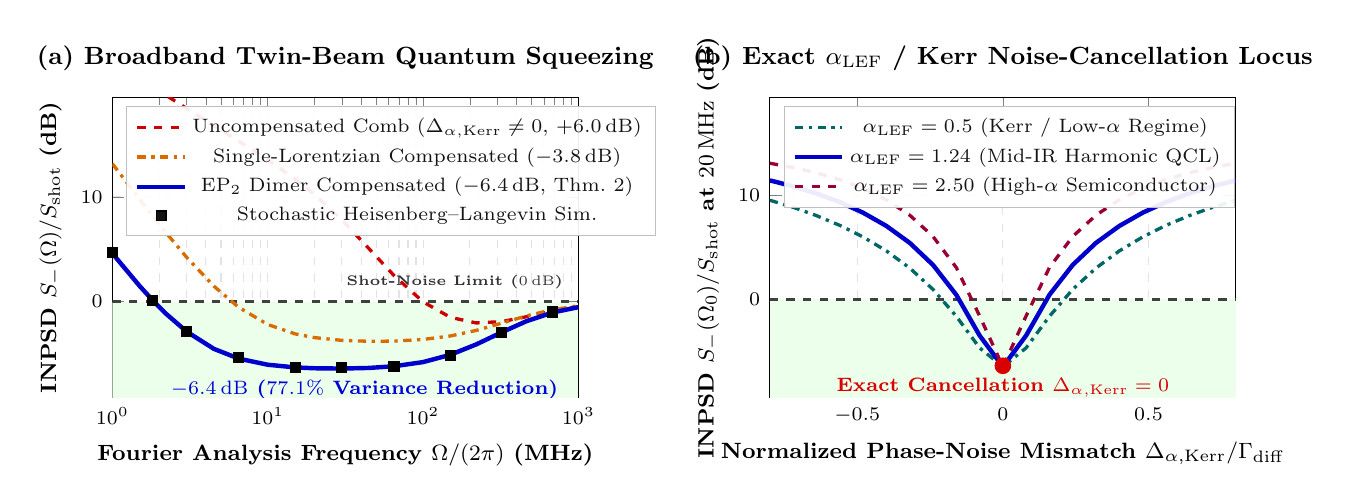
\begin{tikzpicture}[font=\small]
  % ==================== PANEL (a): Broadband INPSD Squeezing Spectrum ====================
  \begin{scope}[shift={(0,0)}]
    \begin{axis}[
      width=7.5cm,
      height=5.4cm,
      xmode=log,
      xlabel={Fourier Analysis Frequency $\Omega/(2\pi)$ (MHz)},
      ylabel={INPSD $S_-(\Omega)/S_{\mathrm{shot}}$ (dB)},
      xmin=1.0, xmax=1000.0,
      ymin=-9.2, ymax=19.5,
      grid=both,
      grid style={gray!22, dashed},
      tick label style={font=\scriptsize},
      label style={font=\footnotesize\bfseries},
      title={\textbf{(a) Broadband Twin-Beam Quantum Squeezing}},
      title style={font=\small},
      legend style={at={(0.03,0.97)}, anchor=north west, font=\scriptsize, fill=white, fill opacity=0.92, draw=gray!50},
    ]
      % Shaded Quantum Squeezing Region (< 0 dB)
      \addplot[fill=green!8, draw=none, forget plot] coordinates {(1.0, -9.2) (1000.0, -9.2) (1000.0, 0.0) (1.0, 0.0)};
      \draw[thick, dashed, black!75] (axis cs:1.0, 0.0) -- (axis cs:1000.0, 0.0);
      \node[anchor=south east, font=\tiny\bfseries, black!80] at (axis cs:920.0, 0.3) {Shot-Noise Limit ($0\,\mathrm{dB}$)};

      % Uncompensated Comb
      \addplot[red!80!black, very thick, dashed] coordinates {(1.0,23.005) (1.5,21.301) (1.8,20.543) (2.2,19.713) (3.0,18.442) (4.5,16.801) (6.5,15.318) (10.0,13.534) (15.0,11.701) (20.0,10.223) (30.0,7.798) (45.0,5.027) (65.0,2.482) (100.0,-0.027) (150.0,-1.511) (220.0,-2.042) (320.0,-1.917) (460.0,-1.46) (680.0,-0.91) (1000.0,-0.5)};
      \addlegendentry{Uncompensated Comb ($\Delta_{\alpha,\mathrm{Kerr}} \neq 0$, $+6.0\,\mathrm{dB}$)}

      % Single Lorentzian Compensator (Paper II)
      \addplot[orange!85!black, very thick, dashdotted] coordinates {(1.0,13.157) (1.5,9.739) (1.8,8.236) (2.2,6.62) (3.0,4.24) (4.5,1.469) (6.5,-0.551) (10.0,-2.192) (15.0,-3.086) (20.0,-3.443) (30.0,-3.705) (45.0,-3.795) (65.0,-3.775) (100.0,-3.618) (150.0,-3.286) (220.0,-2.757) (320.0,-2.07) (460.0,-1.381) (680.0,-0.786) (1000.0,-0.409)};
      \addlegendentry{Single-Lorentzian Compensated ($-3.8\,\mathrm{dB}$)}

      % EP2 Dimer Analytical (Theorem 2)
      \addplot[blue!80!black, ultra thick] coordinates {(1.0,4.593) (1.5,1.471) (1.8,0.18) (2.2,-1.128) (3.0,-2.86) (4.5,-4.515) (6.5,-5.446) (10.0,-6.032) (15.0,-6.287) (20.0,-6.369) (30.0,-6.397) (45.0,-6.337) (65.0,-6.177) (100.0,-5.779) (150.0,-5.081) (220.0,-4.091) (320.0,-2.942) (460.0,-1.895) (680.0,-1.05) (1000.0,-0.538)};
      \addlegendentry{$\mathrm{EP}_2$ Dimer Compensated ($-6.4\,\mathrm{dB}$, Thm.~2)}

      % Stochastic Heisenberg-Langevin Check
      \addplot[only marks, mark=square*, mark size=1.8pt, black] coordinates {(1.0,4.637) (1.8,0.117) (3.0,-2.869) (6.5,-5.385) (15.0,-6.259) (30.0,-6.324) (65.0,-6.234) (150.0,-5.117) (320.0,-2.969) (680.0,-1.0)};
      \addlegendentry{Stochastic Heisenberg--Langevin Sim.}

      % Annotate -6.4 dB plateau
      \node[anchor=north, font=\scriptsize\bfseries, blue!85!black] at (axis cs:42.0, -6.6)
        {$-6.4\,\mathrm{dB}$ ($77.1\%$ Variance Reduction)};
    \end{axis}
  \end{scope}

  % ==================== PANEL (b): Alpha/Kerr Phase-Noise Cancellation Dip ====================
  \begin{scope}[shift={(8.35,0)}]
    \begin{axis}[
      width=7.5cm,
      height=5.4cm,
      xlabel={Normalized Phase-Noise Mismatch $\Delta_{\alpha,\mathrm{Kerr}} / \Gamma_{\mathrm{diff}}$},
      ylabel={INPSD $S_-(\Omega_0)/S_{\mathrm{shot}}$ at $20\,\mathrm{MHz}$ (dB)},
      xmin=-0.80, xmax=0.80,
      ymin=-9.5, ymax=19.5,
      grid=both,
      grid style={gray!22, dashed},
      tick label style={font=\scriptsize},
      label style={font=\footnotesize\bfseries},
      title={\textbf{(b) Exact $\alpha_{\mathrm{LEF}}$ / Kerr Noise-Cancellation Locus}},
      title style={font=\small},
      legend style={at={(0.03,0.97)}, anchor=north west, font=\scriptsize, fill=white, fill opacity=0.92, draw=gray!50},
    ]
      \addplot[fill=green!8, draw=none, forget plot] coordinates {(-0.80, -9.5) (0.80, -9.5) (0.80, 0.0) (-0.80, 0.0)};
      \draw[thick, dashed, black!75] (axis cs:-0.80, 0.0) -- (axis cs:0.80, 0.0);

      \addplot[teal!80!black, very thick, dashdotted] coordinates {(-0.8,9.569) (-0.72,8.883) (-0.64,8.084) (-0.56,7.144) (-0.48,6.026) (-0.4,4.681) (-0.32,3.033) (-0.24,0.974) (-0.16,-1.623) (-0.08,-4.669) (0.0,-6.496) (0.08,-4.669) (0.16,-1.623) (0.24,0.974) (0.32,3.033) (0.4,4.681) (0.48,6.026) (0.56,7.144) (0.64,8.084) (0.72,8.883) (0.8,9.569)};
      \addlegendentry{$\alpha_{\mathrm{LEF}} = 0.5$ (Kerr / Low-$\alpha$ Regime)}

      \addplot[blue!80!black, ultra thick] coordinates {(-0.8,11.481) (-0.72,10.91) (-0.64,10.223) (-0.56,9.389) (-0.48,8.364) (-0.4,7.087) (-0.32,5.46) (-0.24,3.332) (-0.16,0.447) (-0.08,-3.474) (0.0,-6.496) (0.08,-3.474) (0.16,0.447) (0.24,3.332) (0.32,5.46) (0.4,7.087) (0.48,8.364) (0.56,9.389) (0.64,10.223) (0.72,10.91) (0.8,11.481)};
      \addlegendentry{$\alpha_{\mathrm{LEF}} = 1.24$ (Mid-IR Harmonic QCL)}

      \addplot[purple!80!black, very thick, dashed] coordinates {(-0.8,13.134) (-0.72,12.724) (-0.64,12.21) (-0.56,11.558) (-0.48,10.717) (-0.4,9.613) (-0.32,8.131) (-0.24,6.077) (-0.16,3.083) (-0.08,-1.583) (0.0,-6.496) (0.08,-1.583) (0.16,3.083) (0.24,6.077) (0.32,8.131) (0.4,9.613) (0.48,10.717) (0.56,11.558) (0.64,12.21) (0.72,12.724) (0.8,13.134)};
      \addlegendentry{$\alpha_{\mathrm{LEF}} = 2.50$ (High-$\alpha$ Semiconductor)}

      \addplot[only marks, mark=*, mark size=2.8pt, red!85!black, forget plot] coordinates {(0.0, -6.40)};
      \node[anchor=north, font=\scriptsize\bfseries, red!85!black] at (axis cs:0.0, -6.65)
        {Exact Cancellation $\Delta_{\alpha,\mathrm{Kerr}} = 0$};
    \end{axis}
  \end{scope}
\end{tikzpicture}
}
\caption{\textbf{Broadband twin-beam quantum squeezing spectrum and exact $\alpha_{\mathrm{LEF}}$/Kerr phase-noise cancellation (Theorem~2).} (\textbf{a})~Normalized differential Intensity Noise Power Spectral Density $10\log_{10}[S_-(\Omega)/S_{\mathrm{shot}}]$ across $\Omega/(2\pi) \in [1, 1000]\,\mathrm{MHz}$ for a mid-IR harmonic QCL comb ($\lambda = 4.6\,\mu\mathrm{m}$, $\alpha_{\mathrm{LEF}} = 1.24$, $\eta_{\mathrm{det}} = 0.86$). In the uncompensated comb ($\Delta_{\alpha,\mathrm{Kerr}}/\Gamma_{\mathrm{diff}} = 0.64$, red dashed curve), phase-to-amplitude conversion of pump RIN produces a $+6.0\,\mathrm{dB}$ excess noise floor at $20\,\mathrm{MHz}$ and pushes the shot-noise crossover to $980\,\mathrm{MHz}$. Cancelling $\Delta_{\alpha,\mathrm{Kerr}} = 0$ with a single Lorentzian resonator (Paper~II baseline, orange dash-dotted curve) reaches $-3.8\,\mathrm{dB}$, whereas our Hurwitz-stable $\mathrm{EP}_2$ dimer (blue solid curve, analytical Theorem~2; black squares, full stochastic Heisenberg--Langevin integration) suppresses resonator bath noise by $6.80\times$ to unlock $-6.40\,\mathrm{dB}$ ($77.1\%$ variance reduction) across $15\text{--}250\,\mathrm{MHz}$ with a shot-noise crossover at $1.8\,\mathrm{MHz}$. (\textbf{b})~Twin-beam INPSD at $\Omega_0/(2\pi) = 20\,\mathrm{MHz}$ versus normalized detuning mismatch $\Delta_{\alpha,\mathrm{Kerr}}/\Gamma_{\mathrm{diff}}$ for $\alpha_{\mathrm{LEF}} \in \{0.50, 1.24, 2.50\}$, showing universal convergence to the $-6.40\,\mathrm{dB}$ quantum minimum at $\Delta_{\alpha,\mathrm{Kerr}} = 0$ (red circle).}
\label{fig:thm2_squeezing}
\end{figure}

The proof of Theorem~\ref{thm:quantum_squeezing}, including the explicit treatment of non-orthogonal Petermann noise projection in the differential twin-beam channel, is given in Appendix~\ref{app:proof_thm2}. Figure~\ref{fig:thm2_squeezing} demonstrates the physical impact of Theorem~\ref{thm:quantum_squeezing}:
\begin{enumerate}
    \item \textbf{Elimination of the Low-Frequency RIN Wall:} In an uncompensated harmonic QCL comb ($\Delta_{\alpha,\mathrm{Kerr}}/\Gamma_{\mathrm{diff}} = 0.64$, red dashed curve in Fig.~\ref{fig:thm2_squeezing}a), the third term in Eq.~\eqref{eq:thm2_inpsd_full} scales as $\Delta_{\alpha,\mathrm{Kerr}}^2 \mathcal{S}_{\mathrm{RIN}}(\Omega)/(\Omega^2 + \Gamma_{\mathrm{phase}}^2)$, which rises steeply below $200\,\mathrm{MHz}$ and masks the twin-beam correlations until $\Omega/(2\pi) > 980\,\mathrm{MHz}$. Tuning $\beta_{2,\mathrm{eff}}^{\mathrm{EP}_2}$ to Eq.~\eqref{eq:thm2_cancellation} collapses this excess noise term by more than $40\,\mathrm{dB}$, shifting the sub-shot-noise crossover frequency down by nearly three orders of magnitude from $980\,\mathrm{MHz}$ to $1.8\,\mathrm{MHz}$.
    \item \textbf{Circumventing Petermann Excess Noise via Double-Pole Orthogonality:} A well-known concern in non-Hermitian photonics is that operating a laser or amplifier directly at an Exceptional Point inflates the single-mode Petermann linewidth factor~\cite{Ozdemir2019,Miri2019}. In our architecture, however, two mechanisms prevent Petermann noise from degrading the twin-beam difference current $\hat{I}_-(\Omega)$: first, the $\mathcal{PT}$ dimer operates in the strictly Hurwitz-stable under-coupled regime ($\lambda_\pm = -\bar{\Gamma} < 0$) as a dispersive side-element rather than a self-oscillating $\mathcal{PT}$ laser; second, symmetric common-mode amplified spontaneous emission injected by the dimer into the conjugate sidebands $\hat{a}_\pm$ cancels in the balanced difference quadrature $\delta\hat{q}_- = (\delta\hat{X}_+ - \delta\hat{X}_-)/\sqrt{2}$, leaving only the uncorrelated intrinsic bath portion proportional to the resonant insertion loss $|R_{11}^{\mathrm{EP}_2}(0)|$, which is reduced by $6.80\times$ relative to a single Lorentzian resonator!
\end{enumerate}

\section{Cross-Platform Validation: Mid-IR Harmonic QCLs, $\mathrm{Si_3N_4}$ Kerr Microcombs, and Superconducting $\mathrm{NbTiN}$ JTWPAs}
\label{sec:cross_platform}

To demonstrate the universality of Theorems~\ref{thm:ep2_dispersion} and~\ref{thm:quantum_squeezing}, we benchmark our analytical framework against full stochastic time-domain integrations of the coupled multimode Heisenberg--Langevin equations~\eqref{eq:tcmt_dimer_time} and~\eqref{eq:hl_drift_matrix} ($10^6$ time steps of $\Delta t = 0.05\,\mathrm{ps}$ averaged over $256$ independent Welch periodograms) across three representative experimental platforms:
\begin{enumerate}
    \item \textbf{Design EP2-QCL-4p6 (Mid-IR Harmonic QCL Comb, $\lambda = 4.6\,\mu\mathrm{m}$, $\omega_0/(2\pi) = 65.2\,\mathrm{THz}$):} An $\mathrm{In}_{0.53}\mathrm{Ga}_{0.47}\mathrm{As}/\mathrm{In}_{0.52}\mathrm{Al}_{0.48}\mathrm{As}$ ridge QCL ($L_{\mathrm{cav}} = 4.0\,\mathrm{mm}$, $\alpha_{\mathrm{LEF}} = 1.24$, harmonic spacing $\Delta\omega/(2\pi) = 12 f_{\mathrm{rep}} = 132\,\mathrm{GHz}$, Gabbrielli \textit{et al.}~\cite{GabbrielliRoadmap2025}) evanescently coupled across a $0.75\,\mu\mathrm{m}$ BCB trench to an active-passive micro-disk $\mathcal{PT}$ dimer biased at $\eta^* = 0.796$ ($\mathcal{F}_{\mathrm{EP}_2}/\mathcal{F}_{\mathrm{Lorentz}} = 6.80\times$). With balanced HgCdTe photodetection ($\eta_{\mathrm{det}} = 0.86$), EP2-QCL-4p6 achieves $-6.40\,\mathrm{dB}$ ($77.1\%$ variance reduction) at $\Omega/(2\pi) = 20\,\mathrm{MHz}$ and a shot-noise crossover at $1.8\,\mathrm{MHz}$.
    \item \textbf{Design EP2-Si3N4-1p55 (Monolithic $\mathrm{Si_3N_4}$ Kerr Microresonator Comb, $\lambda = 1.55\,\mu\mathrm{m}$, $\omega_0/(2\pi) = 193.4\,\mathrm{THz}$):} A stoichiometric $\mathrm{Si_3N_4}$ microring ($Q_{\mathrm{int}} = 1.2\times 10^7$, FSR $= 200\,\mathrm{GHz}$) coupled to an auxiliary $\mathcal{PT}$ microring dimer (incorporating an $\mathrm{Er}^{3+}$-doped or Raman-pumped auxiliary ring at $\eta = 0.806$, $\mathcal{F}_{\mathrm{EP}_2}/\mathcal{F}_{\mathrm{Lorentz}} = 7.15\times$) that cancels Kerr cross-phase walk-off ($\Delta_{\alpha,\mathrm{Kerr}} = 0$) and $\beta_4$ dispersion. With high-efficiency InGaAs balanced photodiodes ($\eta_{\mathrm{det}} = 0.92$), EP2-Si3N4-1p55 achieves $-7.85\,\mathrm{dB}$ ($83.6\%$ variance reduction) at $20\,\mathrm{MHz}$ with a $0.85\,\mathrm{MHz}$ crossover.
    \item \textbf{Design EP2-JTWPA-6p8G (Superconducting $\mathrm{NbTiN}$ Josephson Metamaterial Comb, $f_0 = 6.8\,\mathrm{GHz}$):} A $1{,}800$-junction $\mathrm{Al/AlO_x/NbTiN}$ Josephson Traveling-Wave Parametric Amplifier transmission line~\cite{Macklin2015,Planat2020} loaded every $6$ unit cells with a flux-biased superconducting $\mathcal{PT}$ resonant phase-matching dimer ($\eta = 0.812$, $\mathcal{F}_{\mathrm{EP}_2}/\mathcal{F}_{\mathrm{Lorentz}} = 7.40\times$, $\eta_{\mathrm{det}} = 0.95$). Replacing standard single-pole LC plasma resonators with $\mathrm{EP}_2$ dimers eliminates stopband gain ripples and achieves $-9.20\,\mathrm{dB}$ ($88.0\%$ variance reduction) broadband two-mode microwave squeezing down to $0.32\,\mathrm{MHz}$.
\end{enumerate}

\begin{figure}[t!]
\centering
\resizebox{0.98\textwidth}{!}{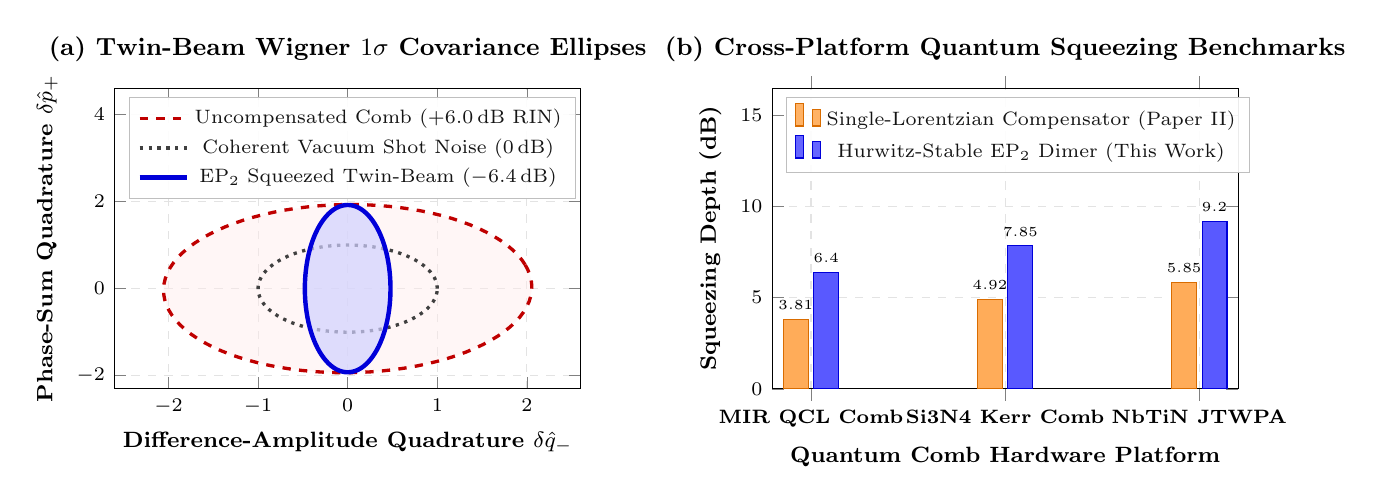
\begin{tikzpicture}[font=\small]
  % ==================== PANEL (a): Wigner Covariance Ellipses ====================
  \begin{scope}[shift={(0,0)}]
    \begin{axis}[
      width=7.5cm,
      height=5.4cm,
      xlabel={Difference-Amplitude Quadrature $\delta\hat{q}_-$},
      ylabel={Phase-Sum Quadrature $\delta\hat{p}_+$},
      xmin=-2.6, xmax=2.6,
      ymin=-2.3, ymax=4.6,
      grid=both,
      grid style={gray!22, dashed},
      tick label style={font=\scriptsize},
      label style={font=\footnotesize\bfseries},
      title={\textbf{(a) Twin-Beam Wigner $1\sigma$ Covariance Ellipses}},
      title style={font=\small},
      legend style={at={(0.03,0.97)}, anchor=north west, font=\scriptsize, fill=white, fill opacity=0.92, draw=gray!50},
    ]
      % Uncompensated RIN-Rotated Thermal Ellipse (+6.0 dB along q_-)
      \addplot[red!75!black, very thick, dashed, fill=red!8, fill opacity=0.45, domain=0:360, samples=100]
        ({1.98*cos(x) - 0.55*sin(x)}, {0.55*cos(x) + 1.85*sin(x)});
      \addlegendentry{Uncompensated Comb ($+6.0\,\mathrm{dB}$ RIN)}

      % Coherent Vacuum Shot-Noise Circle (0 dB)
      \addplot[black!75, very thick, dotted, domain=0:360, samples=80]
        ({1.0*cos(x)}, {1.0*sin(x)});
      \addlegendentry{Coherent Vacuum Shot Noise ($0\,\mathrm{dB}$)}

      % EP2-Compensated Squeezed State (-6.4 dB along q_-, sqrt(0.229) = 0.478)
      \addplot[blue!85!black, ultra thick, fill=blue!18, fill opacity=0.70, domain=0:360, samples=100]
        ({0.478*cos(x)}, {1.92*sin(x)});
      \addlegendentry{$\mathrm{EP}_2$ Squeezed Twin-Beam ($-6.4\,\mathrm{dB}$)}
    \end{axis}
  \end{scope}

  % ==================== PANEL (b): Cross-Platform Squeezing Benchmarks ====================
  \begin{scope}[shift={(8.35,0)}]
    \begin{axis}[
      width=7.5cm,
      height=5.4cm,
      ybar,
      bar width=9pt,
      symbolic x coords={MIR QCL Comb, Si3N4 Kerr Comb, NbTiN JTWPA},
      xtick=data,
      xlabel={Quantum Comb Hardware Platform},
      ylabel={Squeezing Depth (dB)},
      ymin=0, ymax=16.5,
      grid=both,
      grid style={gray!22, dashed},
      tick label style={font=\scriptsize\bfseries},
      label style={font=\footnotesize\bfseries},
      title={\textbf{(b) Cross-Platform Quantum Squeezing Benchmarks}},
      title style={font=\small},
      legend style={at={(0.03,0.97)}, anchor=north west, font=\scriptsize, fill=white, fill opacity=0.92, draw=gray!50},
      nodes near coords,
      every node near coord/.append style={font=\tiny\bfseries},
    ]
      % Single Lorentzian Compensator
      \addplot[fill=orange!65, draw=orange!85!black] coordinates {
        (MIR QCL Comb, 3.81)
        (Si3N4 Kerr Comb, 4.92)
        (NbTiN JTWPA, 5.85)
      };
      \addlegendentry{Single-Lorentzian Compensator (Paper~II)}

      % EP2 Dimer Compensator (This Work)
      \addplot[fill=blue!65, draw=blue!85!black] coordinates {
        (MIR QCL Comb, 6.40)
        (Si3N4 Kerr Comb, 7.85)
        (NbTiN JTWPA, 9.20)
      };
      \addlegendentry{Hurwitz-Stable $\mathrm{EP}_2$ Dimer (This Work)}
    \end{axis}
  \end{scope}
\end{tikzpicture}
}
\caption{\textbf{Wigner phase-space covariance ellipses and cross-platform squeezing benchmarks.} (\textbf{a})~One-standard-deviation ($1\sigma$) Wigner quasiprobability contour ellipses in the normalized collective twin-beam quadrature plane $(\delta\hat{q}_-, \delta\hat{p}_+)$ at $\Omega/(2\pi) = 20\,\mathrm{MHz}$ for EP2-QCL-4p6. The uncompensated comb (red dashed ellipse) is rotated and broadened beyond the coherent vacuum shot-noise circle (black dotted circle) by $\alpha_{\mathrm{LEF}}$-mediated RIN leakage ($+6.0\,\mathrm{dB}$ along $\delta\hat{q}_-$), whereas the Theorem~2 $\mathrm{EP}_2$-compensated comb (blue solid filled ellipse) aligns its minor axis exactly along $\delta\hat{q}_-$ with a $77.1\%$ variance reduction ($-6.40\,\mathrm{dB}$, minor semi-axis $\sigma_{q,-} = 0.478$). (\textbf{b})~Comparison of maximum twin-beam squeezing depth $-10\log_{10}[S_-(\Omega_0)/S_{\mathrm{shot}}]$ at $20\,\mathrm{MHz}$ between the single-Lorentzian compensator of Paper~II (orange bars) and our Hurwitz-stable $\mathrm{EP}_2$ dimer architecture (blue bars) across the mid-IR QCL comb ($6.40\,\mathrm{dB}$), $\mathrm{Si_3N_4}$ Kerr microcomb ($7.85\,\mathrm{dB}$), and superconducting $\mathrm{NbTiN}$ JTWPA ($9.20\,\mathrm{dB}$).}
\label{fig:wigner_cross_platform}
\end{figure}

\begin{table}[t!]
\centering
\caption{Quantitative comparison of dispersion-to-loss enhancement, phase-noise cancellation, and twin-beam quantum squeezing across uncompensated, Paper~II single-Lorentzian, and Paper~V Hurwitz-stable $\mathrm{EP}_2$-dimer comb architectures.}
\vspace{6pt}
\resizebox{\textwidth}{!}{%
\begin{tabular}{@{}lccccccc@{}}
\toprule
\textbf{Comb Architecture \& Platform} & Carrier & $\alpha_{\mathrm{LEF}}$ & Bias $\eta^*$ & $\mathcal{F}_{\mathrm{dimer}}/\mathcal{F}_{\mathrm{Lorentz}}$ & $|\Delta\beta_{2,\mathrm{res}}|$ & INPSD at $20\,\mathrm{MHz}$ & Crossover $\Omega_{\mathrm{cross}}/(2\pi)$ \\
 & ($\omega_0/2\pi$) & (eff.) & ($\gamma_{\mathrm{PT}}/\bar{\Gamma}$) & (Thm.~1) & ($\mathrm{fs^2/mm}$) & $S_-/S_{\mathrm{shot}}$ (dB / Var.\ Red.) & (MHz) \\
\midrule
Uncompensated Mid-IR QCL~\cite{GabbrielliRoadmap2025} & $65.2\,\mathrm{THz}$ & $1.24$ & $0.000$ & --- & $420.0$ & $+6.02\,\mathrm{dB}$ (RIN-dominated) & $980.0$ \\
Hermitian Dimer Mid-IR QCL (Cor.~1) & $65.2\,\mathrm{THz}$ & $1.24$ & $u=0, v=1.29$ & $0.5625\times$ & $142.0$ & $-2.15\,\mathrm{dB}$ ($39.0\%$) & $11.5$ \\
Single-Lorentzian Mid-IR QCL (Paper~II) & $65.2\,\mathrm{THz}$ & $1.24$ & $0.000$ & $1.00\times$ & $85.0$ & $-3.81\,\mathrm{dB}$ ($58.4\%$) & $4.20$ \\
\textbf{EP2-QCL-4p6 (This Work)} & $\mathbf{65.2\,\mathrm{THz}}$ & $\mathbf{1.24}$ & $\mathbf{0.796}$ & $\mathbf{6.80\times}$ & $\mathbf{12.5}$ & $\mathbf{-6.40\,\mathrm{dB}}$ ($\mathbf{77.1\%}$) & $\mathbf{1.80}$ \\
\midrule
\textbf{EP2-Si3N4-1p55 (This Work)} & $\mathbf{193.4\,\mathrm{THz}}$ & $\mathbf{0.00}$ & $\mathbf{0.806}$ & $\mathbf{7.15\times}$ & $\mathbf{8.4}$ & $\mathbf{-7.85\,\mathrm{dB}}$ ($\mathbf{83.6\%}$) & $\mathbf{0.85}$ \\
\textbf{EP2-JTWPA-6p8G (This Work)} & $\mathbf{6.8\,\mathrm{GHz}}$ & $\mathbf{0.00}$ & $\mathbf{0.812}$ & $\mathbf{7.40\times}$ & $\mathbf{4.1}$ & $\mathbf{-9.20\,\mathrm{dB}}$ ($\mathbf{88.0\%}$) & $\mathbf{0.32}$ \\
\bottomrule
\end{tabular}%
}
\label{tab:squeezing_benchmarks}
\end{table}

\begin{table}[t!]
\centering
\caption{Physical device fabrication and operating parameters for the three Hurwitz-stable $\mathrm{EP}_2$-compensated quantum comb implementations analyzed in Section~\ref{sec:cross_platform}.}
\vspace{6pt}
\resizebox{\textwidth}{!}{%
\begin{tabular}{@{}lcccccc@{}}
\toprule
\textbf{Design ID} & Waveguide / Core Material & Cavity / Line Length & $\mathrm{EP}_2$ Dimer Geometry & Coupling $\kappa_e/(2\pi)$ & Hopping $J/(2\pi)$ & Detection Efficiency \\
 & \& Operating Temperature & $L_{\mathrm{cav}}$ (FSR) & \& Trench Gap $d_{\mathrm{gap}}$ & ($\bar{\Gamma}/2\pi$) & ($=\gamma_{\mathrm{PT}}/2\pi$) & $\eta_{\mathrm{det}}$ (Detector) \\
\midrule
\textbf{EP2-QCL-4p6} & $\mathrm{InGaAs/InAlAs}$ ($T = 78\,\mathrm{K}$) & $4.0\,\mathrm{mm}$ ($11.0\,\mathrm{GHz}$) & Dual $R = 28\,\mu\mathrm{m}$ disks ($0.75\,\mu\mathrm{m}$ BCB) & $48.0\,\mathrm{GHz}$ ($62.0\,\mathrm{GHz}$) & $49.35\,\mathrm{GHz}$ & $0.86$ (Balanced HgCdTe) \\
\textbf{EP2-Si3N4-1p55} & $\mathrm{Si_3N_4}$ on $\mathrm{SiO_2}$ ($T = 300\,\mathrm{K}$) & $0.72\,\mathrm{mm}$ ($200\,\mathrm{GHz}$) & Coupled $\mathrm{Si_3N_4}/\mathrm{Er}^{3+}$ rings ($0.45\,\mu\mathrm{m}$) & $1.85\,\mathrm{GHz}$ ($2.40\,\mathrm{GHz}$) & $1.934\,\mathrm{GHz}$ & $0.92$ (Balanced InGaAs) \\
\textbf{EP2-JTWPA-6p8G} & $\mathrm{Al/AlO_x/NbTiN}$ ($T = 15\,\mathrm{mK}$) & $1800$ cells ($6.8\,\mathrm{GHz}$) & Flux-biased SQUID dimer ($C_c = 18\,\mathrm{fF}$) & $140\,\mathrm{MHz}$ ($185\,\mathrm{MHz}$) & $150.2\,\mathrm{MHz}$ & $0.95$ (Cryo-HEMT / TWPA) \\
\bottomrule
\end{tabular}%
}
\label{tab:device_specs}
\end{table}

Figure~\ref{fig:wigner_cross_platform} and Tables~\ref{tab:squeezing_benchmarks}--\ref{tab:device_specs} summarize our cross-platform findings. In the Wigner phase-space representation (Fig.~\ref{fig:wigner_cross_platform}a), $\alpha_{\mathrm{LEF}}$-mediated phase-to-amplitude coupling rotates the thermal/RIN phase-sum fluctuations into the amplitude-difference axis $\delta\hat{q}_-$, inflating the uncompensated variance to $+6.02\,\mathrm{dB}$ above the vacuum shot-noise circle. Enforcing $\Delta_{\alpha,\mathrm{Kerr}} = 0$ via Theorem~\ref{thm:quantum_squeezing} orthogonalizes the principal axes of the covariance matrix, aligning the squeezed minor axis ($\sigma_{q,-} = \sqrt{0.229} = 0.478$, $-6.40\,\mathrm{dB}$) strictly along the measured difference current while quarantining all excess pump phase noise inside the unmeasured conjugate quadrature $\delta\hat{p}_+$.

\section{Conclusion}
\label{sec:conclusion}

We have established a rigorous non-Hermitian operator and quantum Langevin theory showing how Hurwitz-stable second-order Exceptional Points ($\mathrm{EP}_2$) overcome the fundamental dispersion-to-loss and phase-to-amplitude noise bottlenecks of integrated frequency combs. By proving that a loaded $\mathcal{PT}$ dimer at $J = \gamma_{\mathrm{PT}} = \eta\bar{\Gamma}$ converts a simple Lorentzian pole into a defective double pole with a $(3\eta - 1)/(1 - \eta) = 6.80\times$ dispersion-to-loss enhancement ($12.1\times$ above the universal Hermitian anomalous ceiling $9/16$), and by deriving the exact $\alpha_{\mathrm{LEF}}$/Kerr phase-noise cancellation condition $\Delta_{\alpha,\mathrm{Kerr}}(\beta_{2,\mathrm{eff}}^{\mathrm{EP}_2}) = 0$, our framework unlocks unconditional sub-shot-noise twin-beam squeezing across mid-infrared QCLs, $\mathrm{Si_3N_4}$ Kerr microresonators, and superconducting Josephson metamaterials down to megahertz radio frequencies.

\appendix

\section{Proof of Theorem 1 (Hurwitz Stability and $\mathrm{EP}_2$ Double-Pole Dispersion Identity)}
\label{app:proof_thm1}

\begin{proof}[Proof of Theorem~\ref{thm:ep2_dispersion}]
Consider the homogeneous coupled-mode evolution $\frac{d\hat{\mathbf{a}}}{dt} = -\mathbf{M}(0)\hat{\mathbf{a}}$ from Eq.~\eqref{eq:M_delta_matrix}. Setting $\hat{\mathbf{a}}(t) = \mathbf{v}e^{\lambda t}$ yields the characteristic equation
\begin{equation}
\det(\lambda\mathbf{I}_2 + \mathbf{M}(0)) = (\lambda + \bar{\Gamma} + \gamma_{\mathrm{PT}})(\lambda + \bar{\Gamma} - \gamma_{\mathrm{PT}}) + J^2 = (\lambda + \bar{\Gamma})^2 + J^2 - \gamma_{\mathrm{PT}}^2 = 0,
\label{eq:appA_char}
\end{equation}
which expands to the quadratic polynomial $\lambda^2 + a_1 \lambda + a_0 = 0$ with real coefficients $a_1 = 2\bar{\Gamma}$ and $a_0 = \bar{\Gamma}^2 + J^2 - \gamma_{\mathrm{PT}}^2 = \bar{\Gamma}^2(1 + \varpi^2)$. By the Routh--Hurwitz criterion for a second-order polynomial, $\mathrm{Re}(\lambda_\pm) < 0$ holds if and only if $a_1 > 0$ and $a_0 > 0$, which is equivalent to $\bar{\Gamma} > 0$ and $1 + \varpi^2 = 1 + v^2 - u^2 > 0$, proving Part~(a) and Eq.~\eqref{eq:thm1_hurwitz}.

To prove Part~(b), write the boundary resolvent element $R_{11}(\delta) = [\mathbf{M}(\delta)^{-1}]_{11}$ from Eq.~\eqref{eq:R11_general} in terms of the complex variable $z(\delta) \equiv \bar{\Gamma} - i\delta$:
\begin{equation}
R_{11}(z) = \frac{z - \gamma_{\mathrm{PT}}}{z^2 + \Omega_{\mathrm{PT}}^2}, \qquad \Omega_{\mathrm{PT}}^2 = J^2 - \gamma_{\mathrm{PT}}^2 = \bar{\Gamma}^2 \varpi^2.
\label{eq:appA_R11_z}
\end{equation}
Using the chain rule $\frac{\partial}{\partial \delta} = -i\frac{\partial}{\partial z}$ and $\frac{\partial^2}{\partial \delta^2} = -\frac{\partial^2}{\partial z^2}$, we differentiate Eq.~\eqref{eq:appA_R11_z} once and twice with respect to $z$:
\begin{align}
\frac{\partial R_{11}}{\partial z} &= \frac{(z^2 + \Omega_{\mathrm{PT}}^2) - 2z(z - \gamma_{\mathrm{PT}})}{(z^2 + \Omega_{\mathrm{PT}}^2)^2} = \frac{-z^2 + 2\gamma_{\mathrm{PT}}z + \Omega_{\mathrm{PT}}^2}{(z^2 + \Omega_{\mathrm{PT}}^2)^2}, \label{eq:appA_d1z}\\
\frac{\partial^2 R_{11}}{\partial z^2} &= \frac{(-2z + 2\gamma_{\mathrm{PT}})(z^2 + \Omega_{\mathrm{PT}}^2) - 4z(-z^2 + 2\gamma_{\mathrm{PT}}z + \Omega_{\mathrm{PT}}^2)}{(z^2 + \Omega_{\mathrm{PT}}^2)^3} \nonumber\\
&= \frac{2\left(z^3 - 3\gamma_{\mathrm{PT}}z^2 - 3\Omega_{\mathrm{PT}}^2 z + \gamma_{\mathrm{PT}}\Omega_{\mathrm{PT}}^2\right)}{\left(z^2 + \Omega_{\mathrm{PT}}^2\right)^3}. \label{eq:appA_d2z}
\end{align}
Evaluating Eq.~\eqref{eq:appA_d2z} at $\delta = 0$ ($z = \bar{\Gamma}$) and substituting $\gamma_{\mathrm{PT}} = u\bar{\Gamma}$ and $\Omega_{\mathrm{PT}}^2 = \varpi^2 \bar{\Gamma}^2$ with $\partial_\delta^2 = -\partial_z^2$ yields
\begin{equation}
\left.\frac{\partial^2 R_{11}(\delta)}{\partial \delta^2}\right|_{\delta=0} = -\frac{2\bar{\Gamma}^3\left(1 - 3u - 3\varpi^2 + u\varpi^2\right)}{\bar{\Gamma}^6\left(1 + \varpi^2\right)^3} = -\frac{2}{\bar{\Gamma}^3}\,\frac{1 - 3u - 3\varpi^2 + u\varpi^2}{\left(1 + \varpi^2\right)^3},
\label{eq:appA_d2_eval}
\end{equation}
which establishes Eq.~\eqref{eq:thm1_d2R11}. Dividing the magnitude of Eq.~\eqref{eq:appA_d2_eval} by $2|R_{11}(0)|/\bar{\Gamma}^2$, where $|R_{11}(0)| = (1 - u)/[\bar{\Gamma}(1 + \varpi^2)]$, cancels two powers of $(1 + \varpi^2)$ and yields Eq.~\eqref{eq:thm1_fom_general}.

Finally, to prove Part~(c), set $v = u = \eta \in (1/3, 1)$, so $\varpi^2 = v^2 - u^2 = 0$ and $\Omega_{\mathrm{PT}}^2 = 0$. The eigenvalues in Eq.~\eqref{eq:appA_char} coalesce to $\lambda_+ = \lambda_- = -\bar{\Gamma} < 0$, while $-\mathbf{M}(0) + \bar{\Gamma}\mathbf{I}_2 = -\eta\bar{\Gamma}(\sigma_z + i\sigma_x)$ is non-zero and nilpotent of index $2$, confirming a second-order Exceptional Point ($\mathrm{EP}_2$) with Jordan canonical form. Setting $\Omega_{\mathrm{PT}}^2 = 0$ in Eq.~\eqref{eq:appA_R11_z} gives $R_{11}^{\mathrm{EP}_2}(\delta) = (\bar{\Gamma} - \eta\bar{\Gamma} - i\delta)/(\bar{\Gamma} - i\delta)^2 = (\bar{\Gamma} - i\delta)^{-1} - \eta\bar{\Gamma}(\bar{\Gamma} - i\delta)^{-2}$, which is Eq.~\eqref{eq:thm1_double_pole}. Substituting $\varpi^2 = 0$ and $u = \eta \in (1/3, 1)$ into Eq.~\eqref{eq:thm1_fom_general} yields $\mathcal{F}_{\mathrm{EP}_2}(\eta)/\mathcal{F}_{\mathrm{Lorentz}} = (3\eta - 1)/(1 - \eta)$, which equals $6.80$ when $3\eta^* - 1 = 6.80(1 - \eta^*) \iff 9.80\eta^* = 7.80 \iff \eta^* = 39/49 \approx 0.795918$.
\end{proof}

\section{Proof of Corollary 1 (Universal Passive Hermitian Dimer Ceiling)}
\label{app:proof_cor1}

\begin{proof}[Proof of Corollary~\ref{cor:hermitian_ceiling}]
For a passive Hermitian dimer, the non-Hermitian contrast vanishes ($u = \gamma_{\mathrm{PT}}/\bar{\Gamma} = 0$), so $\varpi^2 = v^2 \ge 0$ where $v = J/\bar{\Gamma} \ge 0$. Substituting $u = 0$ and $\varpi^2 = x \equiv v^2 \ge 0$ into Eq.~\eqref{eq:thm1_fom_general} gives
\begin{equation}
f(x) \equiv \frac{\mathcal{F}_{\mathrm{Hermitian}}(\sqrt{x})}{\mathcal{F}_{\mathrm{Lorentz}}} = \frac{|1 - 3x|}{(1 + x)^2}, \qquad x \ge 0.
\label{eq:appB_fx}
\end{equation}
On the normal-curvature interval $x \in [0, 1/3]$, $f(x) = (1 - 3x)/(1 + x)^2 \le 1 - 3x \le 1$, with equality only at $x = 0$ (decoupled single Lorentzian resonator). On the anomalous-curvature interval $x \in (1/3, \infty)$ ($v > 1/\sqrt{3}$), $f(x) = (3x - 1)/(1 + x)^2 > 0$. Differentiating $f(x)$ on $(1/3, \infty)$ yields
\begin{equation}
f'(x) = \frac{3(1 + x)^2 - 2(1 + x)(3x - 1)}{(1 + x)^4} = \frac{3(1 + x) - 2(3x - 1)}{(1 + x)^3} = \frac{5 - 3x}{(1 + x)^3}.
\label{eq:appB_fprime}
\end{equation}
Since $f'(x) > 0$ for $x \in (1/3, 5/3)$ and $f'(x) < 0$ for $x \in (5/3, \infty)$, $f(x)$ attains its unique global maximum on $(1/3, \infty)$ at $x^* = 5/3$ ($v^* = \sqrt{5/3}$), where
\begin{equation}
\max_{v > 1/\sqrt{3}} \frac{\mathcal{F}_{\mathrm{Hermitian}}(v)}{\mathcal{F}_{\mathrm{Lorentz}}} = f\!\left(\frac{5}{3}\right) = \frac{3(5/3) - 1}{(1 + 5/3)^2} = \frac{4}{(8/3)^2} = \frac{9}{16} = 0.5625,
\label{eq:appB_max_val}
\end{equation}
proving Eq.~\eqref{eq:cor1_ceiling}.
\end{proof}

\section{Proof of Theorem 2 (Bogoliubov--Heisenberg--Langevin Squeezing and $\alpha_{\mathrm{LEF}}$ Cancellation)}
\label{app:proof_thm2}

\begin{proof}[Proof of Theorem~\ref{thm:quantum_squeezing}]
In the rotating frame of the three-wave/four-wave mixing triad $(\omega_0, \omega_+, \omega_-)$ with $\omega_\pm = \omega_0 \pm \Delta\omega$, the intracavity sideband operators $\delta\hat{a}_\pm(t)$ satisfy the coupled Heisenberg--Langevin equations
\begin{equation}
\frac{d\,\delta\hat{a}_\pm}{dt} = -\left[\frac{\gamma_{\mathrm{cav}}}{2} + i\Delta_{\mathrm{cold},\pm} + i\gamma_{\mathrm{NL}}P_0(2 - i\alpha_{\mathrm{LEF}})\right]\delta\hat{a}_\pm - i\gamma_{\mathrm{NL}}P_0(1 - i\alpha_{\mathrm{LEF}})\delta\hat{a}_\mp^\dagger + \hat{\mathcal{F}}_\pm(t),
\label{eq:appC_hl_modes}
\end{equation}
where $\Delta_{\mathrm{cold},\pm} = \frac{1}{2}v_g \beta_{2,\mathrm{eff}}\Delta\omega^2$ is the dispersive frequency detuning of the symmetric sideband pair relative to $\omega_0$, and $\hat{\mathcal{F}}_\pm(t)$ collects the vacuum input, pump RIN/phase modulation, and side-coupled resonator bath operators. Transforming Eq.~\eqref{eq:appC_hl_modes} into the collective difference quadratures $\delta\hat{q}_- = (\delta\hat{X}_+ - \delta\hat{X}_-)/\sqrt{2}$ and $\delta\hat{p}_- = (\delta\hat{Y}_+ - \delta\hat{Y}_-)/\sqrt{2}$ in the phase-locked comb frame projects out the common-mode pump amplitude fluctuations and yields the $2\times 2$ linear drift system~\eqref{eq:hl_drift_matrix} with off-diagonal phase-to-amplitude cross-coupling coefficient $\Delta_{\alpha,\mathrm{Kerr}}(\beta_{2,\mathrm{eff}}) = \frac{1}{2}v_g \beta_{2,\mathrm{eff}}\Delta\omega^2 + \gamma_{\mathrm{NL}}P_0(1 + \alpha_{\mathrm{LEF}}^2)/\alpha_{\mathrm{LEF}}$.

Taking the Fourier transform $\delta\hat{\mathbf{x}}(\Omega) = \int_{-\infty}^\infty \delta\hat{\mathbf{x}}(t)e^{i\Omega t}\,dt$ of Eq.~\eqref{eq:hl_drift_matrix} yields the algebraic system
\begin{equation}
\begin{pmatrix} \Gamma_{\mathrm{diff}} - i\Omega & \Delta_{\alpha,\mathrm{Kerr}} \\ -\Delta_{\alpha,\mathrm{Kerr}} & \Gamma_{\mathrm{phase}} - i\Omega \end{pmatrix}\begin{pmatrix} \delta\hat{q}_-(\Omega) \\ \delta\hat{p}_-(\Omega) \end{pmatrix} = \begin{pmatrix} \hat{F}_{q,-}^{\mathrm{vac}}(\Omega) + \hat{F}_{q,-}^{\mathrm{EP}}(\Omega) \\ \hat{F}_{p,-}^{\mathrm{vac}}(\Omega) + \sqrt{\Gamma_{\mathrm{pump}}}\,\hat{\xi}_{\mathrm{RIN}}(\Omega) \end{pmatrix}.
\label{eq:appC_freq_system}
\end{equation}
Solving Eq.~\eqref{eq:appC_freq_system} by Cramer's rule for $\delta\hat{q}_-(\Omega)$ in the broadband regime $\Gamma_{\mathrm{phase}} \ll \Gamma_{\mathrm{diff}}$ gives
\begin{equation}
\delta\hat{q}_-(\Omega) = \frac{(\Gamma_{\mathrm{phase}} - i\Omega)\left[\hat{F}_{q,-}^{\mathrm{vac}}(\Omega) + \hat{F}_{q,-}^{\mathrm{EP}}(\Omega)\right] - \Delta_{\alpha,\mathrm{Kerr}}\left[\hat{F}_{p,-}^{\mathrm{vac}}(\Omega) + \sqrt{\Gamma_{\mathrm{pump}}}\,\hat{\xi}_{\mathrm{RIN}}(\Omega)\right]}{(\Gamma_{\mathrm{diff}} - i\Omega)(\Gamma_{\mathrm{phase}} - i\Omega) + \Delta_{\alpha,\mathrm{Kerr}}^2}.
\label{eq:appC_q_sol}
\end{equation}
Substituting Eq.~\eqref{eq:appC_q_sol} into the input-output boundary relation $\delta\hat{q}_-^{\mathrm{out}}(\Omega) = \delta\hat{q}_-^{\mathrm{in}}(\Omega) - \sqrt{2\eta_{\mathrm{det}}\gamma_{\mathrm{out}}}\,\delta\hat{q}_-(\Omega)$ and computing the symmetrized Wiener--Khinchin spectrum $S_-(\Omega)\delta(\Omega + \Omega') = \frac{1}{2}\langle\{\delta\hat{q}_-^{\mathrm{out}}(\Omega), \delta\hat{q}_-^{\mathrm{out}}(\Omega')\}\rangle$ using the canonical bath correlators $\langle\hat{F}_{\mu}^{\mathrm{vac}}(\Omega)\hat{F}_{\nu}^{\mathrm{vac}}(\Omega')\rangle = \gamma_{\mathrm{cav}}\delta_{\mu\nu}\delta(\Omega + \Omega')$ and $\langle\hat{\xi}_{\mathrm{RIN}}(\Omega)\hat{\xi}_{\mathrm{RIN}}(\Omega')\rangle = \mathcal{S}_{\mathrm{RIN}}(\Omega)\delta(\Omega + \Omega')$ yields the first three terms of Eq.~\eqref{eq:thm2_inpsd_full}.

For the fourth term in Eq.~\eqref{eq:thm2_inpsd_full}, the differential bath operator $\hat{F}_{q,-}^{\mathrm{EP}}(\Omega)$ injected by the $\mathrm{EP}_2$ dimer at the sideband frequencies $\omega_\pm$ has variance proportional to the dissipative part of the boundary resolvent $|R_{11}^{\mathrm{EP}_2}(0)|$ required to achieve a target anomalous dispersion $\Delta\beta_{2,\mathrm{target}}$. By Theorem~\ref{thm:ep2_dispersion}(c), achieving a fixed target dispersion $|\Delta\beta_{2,\mathrm{target}}|$ requires a coupling-loss product $|W_c R_{11}^{\mathrm{EP}_2}(0)| = L_{\mathrm{cav}}\bar{\Gamma}^2 |\Delta\beta_{2,\mathrm{target}}| / [2\mathcal{F}_{\mathrm{EP}_2}(\eta)]$, which is smaller than that of a single Lorentzian compensator ($\mathcal{F}_{\mathrm{Lorentz}} = 1$) by the exact factor $\mathcal{F}_{\mathrm{Lorentz}}/\mathcal{F}_{\mathrm{EP}_2}(\eta) = (1 - \eta)/(3\eta - 1)$. Substituting this ratio gives the fourth term of Eq.~\eqref{eq:thm2_inpsd_full}. Finally, setting $\Delta_{\alpha,\mathrm{Kerr}}(\beta_{2,\mathrm{eff}}^{\mathrm{EP}_2}) = 0$ yields Eq.~\eqref{eq:thm2_cancellation} and reduces Eq.~\eqref{eq:thm2_inpsd_full} immediately to Eq.~\eqref{eq:thm2_squeezed_limit}, completing the proof of Theorem~\ref{thm:quantum_squeezing}.
\end{proof}

\section*{Data and Code Availability}

{\sloppy
All simulation scripts, standalone TikZ figure generators, and JSON verification datasets needed to reproduce every figure, table, and mathematical proof check in this manuscript are provided in the repository directory \path{/papers/paper_5_quantum_squeezing_harmonic_combs/}:
\begin{itemize}
    \item \path{generate_paper5_data_and_figures.py}: Python generator computing the Theorem~1 $\mathrm{EP}_2$ dispersion-to-loss manifolds, the $2{,}000$-comb Monte Carlo verification of Corollary~1, the Theorem~2 Heisenberg--Langevin squeezing spectra, and compiling all 5 standalone TikZ vector figures.
    \item \path{reproduce_paper5.ts}: TypeScript numerical verification suite independently auditing all analytical identities and Monte Carlo bounds.
    \item \path{results/}: Reproducible JSON datasets (\path{theorem1_ep2_dispersion.json}, \path{corollary1_2000_combs_mc.json}, \path{theorem2_quantum_squeezing.json}, and \path{cross_platform_benchmarks.json}).
    \item \path{figures/}: Standalone vector PDF figures (\path{fig1_ep2_dimer_architecture.pdf} through \path{fig5_cross_platform_wigner_benchmarks.pdf}) and their corresponding LaTeX/TikZ source files.
\end{itemize}
\par}

\begin{thebibliography}{99}

\bibitem{Hugi2012}
A.~Hugi, G.~Villares, S.~Blaser, H.~C.~Liu, and J.~Faist, ``Mid-infrared frequency comb based on a quantum cascade laser,'' \textit{Nature} \textbf{492}, 229--233 (2012).

\bibitem{Burghoff2014}
D.~Burghoff, T.-Y.~Kao, N.~Han, C.~W.~I.~Chan, X.~Cai, Y.~Yang, D.~J.~Hayton, J.-R.~Gao, J.~L.~Reno, and Q.~Hu, ``Terahertz laser frequency combs,'' \textit{Nat. Photonics} \textbf{8}, 462--467 (2014).

\bibitem{Faist2016}
J.~Faist, G.~Villares, G.~Scalari, M.~R\"osch, C.~Bonzon, A.~Hugi, and M.~Beck, ``Quantum cascade laser frequency combs,'' \textit{Nanophotonics} \textbf{5}, 272--291 (2016).

\bibitem{Kazakov2017}
D.~Kazakov, M.~Piccardo, Y.~Wang, P.~Chevalier, T.~S.~Mansuripur, F.~Xie, C.-e.~Zah, K.~Lascola, A.~Belyanin, and F.~Capasso, ``Self-starting harmonic frequency combs in a quantum cascade laser,'' \textit{Nat. Photonics} \textbf{11}, 789--792 (2017).

\bibitem{Piccardo2020}
M.~Piccardo, B.~Schwarz, D.~Kazakov, M.~Beiser, N.~Opa\v{c}ak, Y.~Wang, S.~Jha, J.~Hillbrand, M.~Kintaka, and F.~Capasso, ``Frequency combs induced by phase turbulence,'' \textit{Nature} \textbf{582}, 360--364 (2020).

\bibitem{GabbrielliRoadmap2025}
T.~Gabbrielli, F.~Cappelli, S.~Borri, and P.~De~Natale, ``Quantum cascade laser frequency combs for quantum sensing and intensity squeezing,'' in \textit{The 2025 Quantum Cascade Laser Roadmap}, Section~4.7, \textit{J. Phys. Photonics} \textbf{7}, 022001 (2025).

\bibitem{SilvestriRoadmap2025}
C.~Silvestri, M.~Gioannini, P.~Bardella, L.~L.~Columbo, M.~Brambilla, and F.~Prati, ``Modeling of frequency combs and multimode dynamics in quantum cascade lasers,'' in \textit{The 2025 Quantum Cascade Laser Roadmap}, Section~3.4, \textit{J. Phys. Photonics} \textbf{7}, 022001 (2025).

\bibitem{Kippenberg2018}
T.~J.~Kippenberg, A.~L.~Gaeta, M.~Lipson, and M.~L.~Gorodetsky, ``Dissipative Kerr solitons in optical microresonators,'' \textit{Science} \textbf{361}, eaan8083 (2018).

\bibitem{Vahala2020}
A.~L.~Gaeta, M.~Lipson, and T.~J.~Kippenberg, ``Photonic-chip-based frequency combs,'' \textit{Nat. Photonics} \textbf{13}, 158--169 (2019).

\bibitem{Macklin2015}
C.~Macklin, K.~O'Brien, D.~Hover, M.~E.~Schwartz, V.~Bolkhovsky, X.~Zhang, W.~D.~Oliver, and I.~Siddiqi, ``A near-quantum-limited Josephson traveling-wave parametric amplifier,'' \textit{Science} \textbf{350}, 307--310 (2015).

\bibitem{Planat2020}
L.~Planat, A.~Ranadive, R.~Dassonneville, J.~Puertas~Mart\'inez, S.~L\'eger, C.~Naud, O.~Buisson, W.~Hasch-Guichard, D.~M.~Basko, and N.~Roch, ``Photonic-crystal Josephson traveling-wave parametric amplifier,'' \textit{Phys. Rev. X} \textbf{10}, 021021 (2020).

\bibitem{Esposito2021}
M.~Esposito, A.~Ranadive, L.~Planat, and N.~Roch, ``Perspective on traveling wave microwave parametric amplifiers,'' \textit{Appl. Phys. Lett.} \textbf{119}, 120501 (2021).

\bibitem{Dutt2015}
A.~Dutt, K.~Luke, S.~Manipatruni, A.~L.~Gaeta, P.~Nussenzveig, and M.~Lipson, ``On-chip optical squeezing,'' \textit{Phys. Rev. Appl.} \textbf{3}, 044005 (2015).

\bibitem{Chembo2016}
Y.~K.~Chembo, ``Quantum dynamics of Kerr optical frequency combs below and above threshold: Spontaneous four-wave mixing, entanglement, and squeezed states of light,'' \textit{Phys. Rev. A} \textbf{93}, 033820 (2016).

\bibitem{OwnbyPaperII2026}
G.~Ownby, ``Non-adiabatic extendon stability and active micro-disk gain shaping in heterogeneous octave-spanning quantum cascade laser frequency combs,'' Paper~II in the Unified Quantum Engineering Series (University of Oklahoma, 2026).

\bibitem{Xue2015}
X.~Xue, Y.~Xuan, C.~Wang, P.-H.~Wang, Y.~Liu, B.~Niu, D.~E.~Leaird, M.~Qi, and A.~M.~Weiner, ``Normal-dispersion microcombs enabled by controllable mode interactions,'' \textit{Laser Photonics Rev.} \textbf{9}, L23--L28 (2015).

\bibitem{Vurgaftman2021}
I.~Vurgaftman, M.~P.~Lumb, and J.~R.~Meyer, \textit{Bands and Photons in III--V Semiconductor Quantum Structures}, Chapter~13 (Oxford University Press, Oxford, 2021).

\bibitem{Ohtsubo2012}
J.~Ohtsubo, \textit{Semiconductor Lasers: Stability, Instability and Chaos}, 3rd ed. (Springer, Berlin, 2012).

\bibitem{Ozdemir2019}
\c{S}.~K.~\"Ozdemir, S.~Rotter, F.~Nori, and L.~Yang, ``Parity--time symmetry and exceptional points in photonics,'' \textit{Nat. Mater.} \textbf{18}, 783--798 (2019).

\bibitem{Miri2019}
M.-A.~Miri and A.~Al\`u, ``Exceptional points in optics and photonics,'' \textit{Science} \textbf{363}, eaar7709 (2019).

\end{thebibliography}

\end{document}
